\input{mintmod_eng.tex}
\MPragma{MathSkip}

%\Mtikzexternalize

\begin{document}
\selectlanguage{english}

\MSection{Elementary Arithmetic}
\MLabel{VBKM01}
\MSetSectionID{VBKM01} % wird fuer tikz-Dateien verwendet



\begin{MSectionStart}
\MDeclareSiteUXID{VBKM01_START}
This module provides the mathematical basics to elementary arithmetic and introduces and explains the 
notation used throughout this online course. This module consists of

\begin{itemize}
\item{Section \MNRef{M01_Zahlenbereiche}: \MSRef{M01_Zahlenbereiche}{Numbers, Variables, Terms},}
\item{Section \MNRef{M01_Bruchrechnung}: \MSRef{M01_Bruchrechnung}{Fractional Arithmetic},}
\item{Section \MNRef{M01_Umformen}: \MSRef{M01_Umformen}{Transformation of Terms},}
\item{Section \MNRef{M01_Potenzenwurzeln}: \MSRef{M01_Potenzenwurzeln}{Powers and Roots}, }
\item{and the \MSRef{M01_Ausgangstest}{Final Test}: \MNRef{M01_Ausgangstest}.}
\end{itemize}


\end{MSectionStart}

\MSubsection{Numbers, Variables, Terms}
\MLabel{M01_Zahlenbereiche}

\begin{MIntro}
\MDeclareSiteUXID{VBKM01_ZahlenIntro}

%Einfügung Mengenschreibweise
Mathematics is a science, in which abstract structures and their logical correlations are investigated in general. 
Before we examine the actual subjects of this section in more detail, we shall refer shortly to the fundamental 
notion of a \MEntry{set}{set}. 

\begin{MInfo}
To be able to make statements on a number of structurally similar objects in compact manner such objects 
can be gathered into sets serving as a container for the objects. Let the objects be denoted by $a,b,c,\ldots$, 
then the symbol $M=\{a\MElSetSep b \MElSetSep c \MElSetSep \ldots\}$ forms the set $M$, which contains the previously 
listed objects as \textbf{elements}. The latter statement is written shortly as $a\in M$, $b\in M$, $c\in M$ etc; thus the symbol 
``$\in$'' reads ``is element of''. (Sometimes it is more convenient to reverse the order of element 
and set. To obtain the same statement(s) the symbol $\in$ is turned, e.g.\ $M\ni a$, $M\ni b$, $M\ni c$ etc.\ then 
means the same as before, where ``$\ni$'' now reads ``contains as an element'' or 
``contains''.) 

Apart from the listing notation for sets other notations exist. If, for example, the elements have to fulfil a 
condition $B$, then this is written in the form $T=\{x\MCondSetSep x\MBlank\text{fulfils}\MBlank B\}$. If $x$ is taken (explicitly) from a 
more comprehensive set $U$, then this is also written in the form $T=\{x\MCondSetSep x\in U \MBlank\text{and}\MBlank 
x\MBlank\text{fulfils}\MBlank B\}$ or in short $T=\{x\in U\MCondSetSep x\MBlank\text{fulfils}\MBlank B\}$.
%%Da die Bedingung $B$ eine Einschränkung für die Elemente von $U$ darstellt,
%%ist $T$ dann in natürlicher Weise eine \textbf{Teilmenge} von $U$,
%%notiert in Formelnotation als $T\subset U$.

Statements like ``$x\in U$'' or ``$x\MBlank\text{fulfils}\MBlank B$'' are statements in a 
mathematical sense, e.g.\ you can assign them a unique truth value ``true'' or ``false''. 
Let $A_1$ and $A_2$ be such statements. In the case, that both $A_1$ and $A_2$ are to hold, which means $A_1$ 
\textbf{and} $A_2$ are to hold, this is also written as $A_1 \wedge A_2$. In the case, that only one of the two 
statements needs to hold, i.e.\ $A_1$ \textbf{or} $A_2$ (or both) are to hold, one also writes $A_1\vee A_2$.

For two sets $M$ and $N$ one writes
\begin{itemize}
\item{%
$M\subseteq N$, i.e.\ $M$ is a (improper) \textbf{subset} of $N$, if every element of $M$ is also contained in 
$N$. If at least one element exists that is not contained in $M$, meaning that $M$ is a proper subset of $N$, 
one (also) writes $M\subset N$;
}
\item{%
$M\cup N$ for the \textbf{union} of the two sets; the union denotes the set containing all elements that are at 
least contained in one of the two sets;
}
\item{%
$M\cap N$ for the \textbf{intersection} of the two sets; the intersection denotes the set containing all elements 
that are contained in both of the two sets;
}
\item{%
$N\MSetminus M$ for the \textbf{complement}, i.e.\ the set containing all elements of $N$ that are \textit{not} contained in $M$.
}
\end{itemize}
Thus the union mentioned above is characterised by elements that fulfil the condition $(x\in M) \vee (x\in N)$. However, for
the elements of the intersection $(x\in M) \wedge (x\in N)$ holds. In contrast, the complement above contains such 
elements for which $(x\in N) \wedge (x\notin M)$ holds. The symbol $\notin$ denotes the negation of the element 
statement. 
\end{MInfo}
%

Mathematics involves the world of numbers: 
$$\dots\MElSetSep 0\MElSetSep -3\MElSetSep 4\MElSetSep \Mdfrac{4}{5}\MElSetSep \sqrt 
2\MElSetSep \MEU\MElSetSep \pi\MElSetSep \MZahl{12}{3}\MElSetSep 10^{23}\MElSetSep \dots \MDFPeriod$$ 
\newpage
However, considering different numbers in more detail reveals fundamental differences. Some numbers cannot be 
expressed as a closed decimal fraction, others are almost unimaginable (imaginary), still others can be counted on the 
fingers or can be derived as solutions of equations. 

\begin{MInfo}
The number ranges used throughout this online course are:\ifttm\else\ \\\fi
\begin{tabular}{ll}
$\displaystyle \N=\lbrace 1\MElSetSep 2\MElSetSep 3\MElSetSep\ldots\rbrace$ & the \textbf{set of all natural numbers excluding zero},\\ 
$\displaystyle \N_{0}=\lbrace 0\MElSetSep 1\MElSetSep 2\MElSetSep 3\MElSetSep\ldots\rbrace$ &the \textbf{set of all natural numbers including zero},\\
$\displaystyle \Z=\lbrace \ldots\MElSetSep  -2\MElSetSep -1\MElSetSep 0\MElSetSep 1\MElSetSep 2\MElSetSep \ldots\rbrace$ & the \textbf{set of all integer numbers (integers)},\\
$\displaystyle \Q$ & the \textbf{set of all rational numbers (fractions)},\\
$\displaystyle \R$ & the \textbf{set of all real numbers}.\\ 
\end{tabular}
\end{MInfo}

These number ranges are not independent of each other. They rather form a chain of nested number sets:
$$\N\subset\N_{0}\subset\Z\subset\Q\subset\R \MDFPeriod$$ 
%%Dabei bedeutet das Symbol $\subset$, dass der links stehende Zahlenbereich eine Teilmenge des rechts stehenden Zahlenbereichs ist.
%%Beispielsweise ist jede ganze Zahl aus $\Z$ immer auch eine rationale Zahl aus $\Q$.
One obtains these number ranges by examining the solutions of the following equations and extending the number 
range in such a way that always a solution exists:

\begin{center}
\begin{tabular}{|c|r|r|r|c|}
\hline
Number range & Solvable equation & Unsolvable & Extension by & New range\\
\hline 
$\displaystyle \N$ & $x+2=4$ & $x+2=1$ & negative numbers& $\displaystyle \Z$\\
$\displaystyle \Z$ & $4x=20$ &$4x=5$ & fractions &$\displaystyle \Q$\\
$\displaystyle \Q$ & $x^2=4$ &$x^2=2$ & irrational numbers &$\displaystyle \R$\\
$\displaystyle \R$ & $x^2=2$ &$x^2=-1$ & etc. & \\
\hline
\end{tabular}
\end{center}

Natural numbers occur whenever numbers of objects have to be determined or things have to be numbered. They play a great role 
in combinatorics: the number of possibilities selecting 6 balls out of 49 is, for example, a natural number. In computer science 
natural numbers are the bases of different number systems: the binary system has the base 2, the decimal system has the base 10, 
and the hexadecimal system has the base 16. Specific natural numbers, the prime numbers, form the basis of modern encryption methods. 

Arithmetic on the set of natural numbers is easy, but limits are reached, if you, for example, read a temperature value of 3\,$^\circ$C 
(are plus or minus degrees meant?) or if an equation of the form $x+5=1$ is to be solved. Thus the set of natural numbers has to be extended
by the negative natural numbers to obtain the set of integer numbers $\Z$. The \MEntry{set of integer numbers}{integer numbers $\Z$} is 
denoted by
$$\Z:=\{\dots\MElSetSep  -4\MElSetSep -3\MElSetSep -2\MElSetSep -1\MElSetSep 0\MElSetSep 1\MElSetSep 2\MElSetSep 3\MElSetSep 4\MElSetSep \dots\}.$$
Integer numbers are required whenever the algebraic sign of a natural number is of importance. In $\Z$ numbers can be subtracted from each other 
without any restriction, i.e.\ systems of equations of the form $\displaystyle a+x=b$ are always solvable in $\Z$ ($\displaystyle x=b+(-a)$).

\begin{center}
%-%\MUGraphicsSolo{ganzzahlen.png}{width=10cm}{width:400px}
\MTikzAuto{%
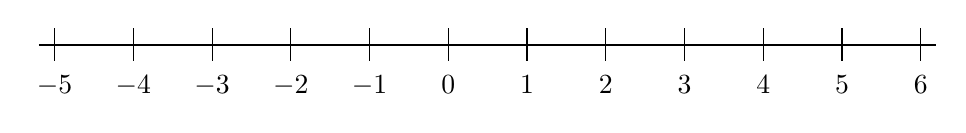
\begin{tikzpicture}[x=1.0cm, y=1.0cm] 
\draw[thick, black] (-5.2,0) -- (6.2,0);
\foreach \x in {-5, -4, ..., 6}
\draw[shift={(\x,0)},color=black] (0pt,6pt) -- (0pt,-6pt) node[below=1.5pt] {\normalsize $\x$};
\end{tikzpicture}
}
\end{center}

On the set of integer numbers a comparing symbol $<$ can be uniquely defined, so that the integer numbers can be ordered into a chain:
$$\dots < -3 < -2 < -1 < 0 < 1 < 2 < 3 < \dots \MDFPeriod$$

\newpage
A rational number is the ratio of two integer numbers:

\begin{MInfo}
The set of \MEntry{rational numbers}{rational numbers $\Q$} is denoted by
$$\Q:=\left\{{\Mdfrac{p}{q}\MCondSetSep p,q\in\Z, q\neq 0 }\right\}.$$
The elements $\displaystyle \Mtfrac{p}{q}$ of the set $\Q$ are called \MEntry{fractions}{fraction}, where $p$ is the 
\MEntry{numerator}{numerator} of the fraction and $q$ is the non-zero \MEntry{denominator}{denominator} of the fraction.
\end{MInfo}
Rational numbers play a role whenever the numerals have to be ``more precise'', i.e.\ if temperatures 
have to be given in fractional amounts of $^\circ$C, portions of surfaces have to be coloured, or medications have to be 
mixed from specific ingredients. 

Note that the representation as a fraction is not unique: one and the same number can be 
represented by several fractions. For example,
$$
2 \;=\; \Mdfrac{4}{2} \;=\; \Mdfrac{1024}{512}
$$
is one and the same rational number.

Also, not every number on the number line can be represented as a fraction. Considering, for example, 
a square with sides of length $1$, the length of the diagonal $d$ can be calculated by means of the 
Pythagorean theorem:

\vspace*{5mm}

\begin{minipage}{0.45\linewidth}
\begin{center}
%-%\MGraphicsSolo{quadrat.png}{width=3cm}
\MTikzAuto{%
\begin{tikzpicture}[x=4.0cm, y=4.0cm] 
\draw[thick, black] (0,0) -- (1,0) -- (1,1) -- (0,1) -- cycle;
\draw[thick, black] (0,1) -- (1,0);
\draw[color=black] (0.5,0.5) node[anchor=south west] {\normalsize $d$};
\draw[stealth'-,black] (0.0,-0.1) -- (0.36,-0.1);
\draw[-stealth',black] (0.65,-0.1) -- (1.0,-0.1);
\draw (0.5,-0.1) node {\scriptsize $1\MEinheit{cm}$};
\end{tikzpicture}
}
\end{center}
\end{minipage}
\begin{minipage}{0.55\linewidth}
\begin{center}
$$d^2 = 1^2+1^2 = 2, \;\mbox{i.e.\ formal}\; d=\sqrt{2}.$$
\end{center}
\end{minipage}

\vspace*{5mm}

Another number, that cannot be represented as a fraction, is obtained by unrolling a wheel of diameter $1$ 
on the number line. The result is the number $\pi$. It can be proven, that these two numbers ($\sqrt{2}$ and $\pi$)
cannot be represented as a fraction. (In the case of $\sqrt{2}$ this proof is relatively simple.) These numbers are two 
example elements of the set of the so called \MEntry{irrational numbers}{irrational numbers}.

\vspace*{5mm}

\begin{center}
%-%\MGraphicsSolo{kreispi.png}{width=10cm}
\MTikzAuto{%
\begin{tikzpicture}[x=2.0cm, y=2.0cm] 
\draw[-stealth',black] (-0.7,0.0) -- (4.0,0.0) node[right=3pt] {$x$};
\draw[color=black] (0,0.5) circle (0.5) ({pi},0.5) circle (0.5);
\draw[-stealth',black] (1.0,0.7) -- (2.14,0.7);
\draw[color=black] (0,3pt) -- (0,-3pt) node[below=2pt] {\small $0$};
\draw[color=black] ({pi},3pt) -- ({pi},-3pt) node[below=2pt] {\small Pi};
\draw[stealth'-,color=black] (0,0.5) ++(20:0.65) arc (20:60:0.65);
\end{tikzpicture}
}
\end{center}

A number is irrational, if it is not rational, i.e. if it cannot be represented as a fraction.
The irrational numbers close the gaps remained so far on the number line, where now every point 
corresponds exactly to one real number. 

\begin{MInfo}
The set of \MEntry{real numbers}{real numbers $\R$} is denoted by $R$ and includes the set of rational 
numbers and the set of irrational numbers. It contains all numbers that can be represented on the number line.
\end{MInfo}

Real numbers serve as measures for lengths, areas, temperatures, masses, etc. Throughout this course 
the mathematical problems are typically solved using real numbers.

A basic property of real numbers is, that they are ordered, i.e. for two real numbers $a,b$ exactly one of
the three relations $a<b$, $a=b$, or $a>b$ holds. Another defining property is the completeness, which -- 
roughly speaking -- describes the ``gaplessness'' of the number line.

\begin{MInfo}
\MLabel{VBKM01_Intervalle}
For two different real numbers, one sometimes considers all numbers lying between these two 
numbers on the number line. Such subsets of real numbers are called \MEntry{intervals}{interval}.
They are described in such a way, that they are assigned a left interval boundary ($a$) and a right 
interval boundary $(b)$ with $a<b$. Depending on whether one interval boundary or two interval 
boundaries are included the following cases exist:


\begin{itemize}
\item{%
$\{x\in\R \MCondSetSep x\ge a \MBlank\text{and}\MBlank x\le b\}
= [a\MIntvlSep b]$ denotes the \textbf{closed} interval
between $a$ and $b$ including the interval boundaries.
}
\item{%
$\{x\in\R \MCondSetSep x> a \MBlank\text{and}\MBlank x< b\}
= \MoIl a\MIntvlSep b\MoIr$ denotes the \textbf{open} interval
between $a$ and $b$ \textit{not including} (excluding) the interval 
boundaries.
}
\item{%
$\{x\in\R \MCondSetSep x\ge a \MBlank\text{and}\MBlank x< b\}
= [a\MIntvlSep b\MoIr$ denotes the \textbf{left-closed and 
right-open} interval between $a$ and $b$, including the left interval boundary but excluding
the right interval boundary.
}
\item{%
$\{x\in\R \MCondSetSep x> a \MBlank\text{and}\MBlank x\le b\}
= \MoIl a\MIntvlSep b]$ denotes the \textbf{left-open and 
right-closed} interval between $a$ and $b$, including the right interval boundary but excluding
the left interval boundary.
}
\end{itemize}
The two last intervals are also called \textbf{half-open}
intervals.

For open interval ends, \textbf{unbounded} intervals can be considered as well. In these cases the 
corresponding condition in the set definition is dropped:
$\{x\in\R \MCondSetSep x\ge a\} = \left[a\MIntvlSep \infty\MoIr[\right]$,
$\{x\in\R \MCondSetSep x> a\} = \MoIl[\left] a\MIntvlSep \infty\MoIr[\right]$,
$\{x\in\R \MCondSetSep x\le b\} = \MoIl[\left] {-}\infty\MIntvlSep b\right]$,
$\{x\in\R \MCondSetSep x< b\} = \MoIl[\left] {-}\infty\MIntvlSep b\MoIr[\right]$,
$\{x\in\R\} = \R = \MoIl[\left] {-}\infty\MIntvlSep \infty\MoIr[\right]$.

Moreover, the following descriptions are common:
$\R^{+}=\MoIl[\left] 0\MIntvlSep \infty\MoIr[\right]$,  
${\R_{0}}^{+}= \left[ 0\MIntvlSep \infty\MoIr[\right]$,  
$\R^{-}=\MoIl[\left] -\infty \MIntvlSep 0\MoIr[\right]$,  
${\R_{0}}^{-}=\MoIl[\left] -\infty \MIntvlSep 0\right]$.  
\end{MInfo}

\end{MIntro}

\begin{MXContent}{Variables and Terms}{Variables and terms}{STD}
\MDeclareSiteUXID{VBKM01_VariablenTerme}

The use of variables, terms, and equations is required to formalise expressions with 
still indeterminate values.

\begin{MInfo}
A \MEntry{variable}{variable} is a symbol (typically a letter) used as a placeholder for an
indeterminate value. A \MEntry{term}{term} is a mathematical expression that can contain variables, arithmetic 
operations and further symbols and, after substituting variables with numbers, gives a specific value. 
Terms can be combined to equations and inequalities, respectively, or they can be inserted into function
descriptions, of which more later.
\end{MInfo}


\begin{MExample}
The textual question 

\textit{In a school class there are four girls more than boys and in total there are 20 children. How many 
girls and boys are in the class, respectively?
}

can be formalised, for example, by introducing the variable $a$ for the number of girls and 
the variable $b$ for the number of boys in the class and setting up the two equations 
$a=b+4$ and $a+b=20$. These equations can be solved by inserting the first equation into 
the second which gives $a=12$ and $b=8$. Out of this, the textual answer 

\textit{In the school class there are $12$ girls and $8$ boys}

can be constructed. Here, for example, $b+4$ is a term, $b$ itself is a variable, and
$a+b=20$ is an equation with a term on the left and a number on the right.
\end{MExample}
Variables (and sometimes also terms) are generally denoted by Latin lowercase letters $x$, $y$, $z$, etc.
Often Greek letters are used as well, for example, if angles are to be separated from numbers.

\begin{MInfo}
\MLabel{VBKM01_Griechisch}
This overview shows the (lowercase and uppercase) letters of the Greek alphabet in 
Greek alphabetical order:
\ \\ \ \\
\begin{tabular}{|*{5}{cc|}}
\ifttm\hline\else\firsthline\fi
%Die Grossbuchstaben, die nicht auch vom lateinischen Alphabet genutzt
%werden, druckt pdfLaTeX aufrecht, MathML dagegen kursiv.
 $\alpha$,       \ifttm$A$\else$\mathrm{A}$\ \ \ \fi & ``alpha''\ \ \ \ \ \ &
 $\beta$,        \ifttm$B$\else$\mathrm{B}$\fi & ``beta''          &
 $\gamma$,       $\Gamma$                      & ``gamma''         &
 $\delta$,       $\Delta$                      & ``delta''         &
 $\Mvarepsilon$, \ifttm$E$\else$\mathrm{E}$\fi & ``epsilon''       \\
 $\zeta$,        \ifttm$Z$\else$\mathrm{Z}$\fi & ``zeta''          &
 $\eta$,         \ifttm$H$\else$\mathrm{H}$\fi & ``eta''           &
 $\vartheta$,    $\Theta$                      & ``theta''         &
 $\iota$,        \ifttm$I$\else$\mathrm{I}$\fi & ``iota''          &
 $\Mvarkappa$,   \ifttm$K$\else$\mathrm{K}$\fi & ``kappa''         \\
 $\lambda$,      $\Lambda$                     & ``lambda''        &
 $\mu$,          \ifttm$M$\else$\mathrm{M}$\fi & ``m\"u''          &
 $\nu$,          \ifttm$N$\else$\mathrm{N}$\fi & ``n\"u''          &
 $\xi$,          $\Xi$                         & ``xi''            &
 $o$,            \ifttm$O$\else$\mathrm{O}$\fi & ``omikron''       \\
 $\pi$,          $\Pi$                         & ``pi''            &
 $\varrho$,      \ifttm$P$\else$\mathrm{P}$\fi & ``rho''           &
 $\sigma$,       $\Sigma$                      & ``sigma''         &
% $\varsigma$,                                  & \dq sigma\dq         &
 $\tau$,         \ifttm$T$\else$\mathrm{T}$\fi & ``tau''          &
 $\upsilon$,     $\Upsilon$                    & ``\"upsilon''     \\
 $\Mvarphi$,     $\Phi$                        & ``phi''           &
 $\chi$,         \ifttm$X$\else$\mathrm{X}$\fi & ``chi''           &
 $\psi$,         $\Psi$                        & ``psi''           &
 $\omega$,       $\Omega$                      & ``omega''         &
 \special{html:&nbsp;}                         & \special{html:&nbsp;}    \\
 \ifttm\hline\else\lasthline\fi
\end{tabular}
\ \\
\MInputHint{In the exercises Greek letters can be entered with their description, e.g.\ \texttt{alpha} instead of $\alpha$.}
\end{MInfo}

It is important, that a term can be evaluated to a specific value, if the variables occurring in the term are substituted 
with numbers:
\newpage
\begin{MExample}
The following expressions are terms:
\begin{itemize}
\item{$x\cdot (y+z)-1$: for $x=1$, $y=2$, and $z=0$ one obtains, for example, the value $1$.}
\item{$\sin(\alpha)+\cos(\alpha)$: for $\alpha=0^\circ$ and $\beta=0^\circ$ one obtains, for example, the value $1$ 
(for the calculation of sine and cosine refer to \MNRef{VBKM05}).}
\item{$1+2+3+4$: no variables occur, however this is a term (which always gives the value $10$).}
\item{$\Mtfrac{\alpha+\beta}{1+\gamma}$: for example, $\alpha=1$, $\beta=2$, and $\gamma=3$ give the value 
$\Mtfrac{3}{4}$. But $\gamma=-1$ is not allowed.}
\item{$\sin(\pi (x+1))$: for example, the term gives always the value zero, if $x$ is substituted with an integer number.}
\item{$z$: a single variable is also a term.}
\item{$1+2+3+\cdots+(n-1)+n$ is a term, in which the variable $n$ occurs in the term itself and defines 
its length as well.}
\end{itemize}
\end{MExample}

\begin{MExample}
These expressions are no terms in a mathematical sense:
\begin{itemize}
\item{$a+b=20$ is an equation (inserting values for $a$ and $b$ gives no number, but the equation is simply true or false).}
\item{$a\cdot (b+c$ is not correctly bracketed,}
\item{``\textit{The ratio of girls in the school class}'' is no term, 
but can be formalised by the term $\Mtfrac{a}{a+b}$,}
\item{$\sin$ is no term but a function name, in contrast $\sin(\alpha)$ is a term (which can be evaluated by 
inserting an angle for $\alpha$).}
\end{itemize}
\end{MExample}

\begin{MExercise}
Given each a term and number values for the occurring variables, what is the evaluation of the term?
\begin{MExerciseItems}
\item{$\Mtfrac{\alpha+\beta}{\alpha-\beta}$ takes the value \MLParsedQuestion{10}{5}{3}{ER1} for $\alpha=6$ and $\beta=4$.}
\item{$y^2+x^2$ takes the value \MLParsedQuestion{10}{2}{3}{ER2} for $y=2x+1$ and $x=-1$.}
\item{$1+2+3+\cdots+(n-1)+n$ takes the value \MLParsedQuestion{10}{21}{3}{ER3} for $n=6$.}
\end{MExerciseItems}
\begin{MHint}{Solution}
Inserting the given values for the variables gives $\Mtfrac{\alpha+\beta}{\alpha-\beta}=\Mtfrac{6+4}{6-4}=\Mtfrac{10}{2}=5$ in a),
$y^2+x^2=(-1)^2+(-1)^2=2$ in b), and $1+2+3+4+5+6=21$ in c).
\end{MHint}
\end{MExercise}

\begin{MExercise}
Formalise, using the given variables, the ratio of girls and the ratio of boys, 
the number of girls being denoted by the variable $a$ and the number of boys by the variable $b$:


The ratio of girls is \MLSimplifyQuestion{15}{a/(a+b)}{5}{a,b}{5}{512}{LSFF1} and
the ratio of boys is \MLSimplifyQuestion{15}{b/(a+b)}{5}{a,b}{5}{512}{LSFF2}.\\
\MInputHint{Fractions can be entered using the slash (above the 7-key on most keyboards), where 
numerator and denominator, respectively, should be bracketed if arithmetic operations occur. The
fraction $\Mtfrac{1+x}{2+y}$ can be entered, for example, by \texttt{(1+x)/(2+y)}.}

\begin{MHint}{Solution}
The total number of children is $a+b$, hence the ratio of girls is $\Mtfrac{a}{a+b}$
and the ratio of boys is $\Mtfrac{b}{a+b}$.
\end{MHint}
\end{MExercise}


Terms can be inserted into each other as well:

\begin{MInfo}
When \MEntry{inserting}{inserting (terms)} terms, a term is inserted instead of a symbol into another term, where the 
replaced symbol has to be bracketed in advance, if the term to be inserted contains several expressions.
\end{MInfo}

\begin{MExample}
Inserting, for example, the value $x=1+2+3$ into the term $x^2+y^2$ gives the new term 
$x^2+y^2=(1+2+3)^2+y^2=36+y^2$ and certainly not $1+2+3^2+y^2=12+y^2$.
\end{MExample}

\begin{MExercise}
Which term is formed, if the following object is inserted into the term $x^2+y^2$:
\begin{MExerciseItems}
\item{The angle $\alpha$ both for $x$ and $y$: Then \MEquationItem{$x^2+y^2$}{\MLFunctionQuestion{13}{2*alpha^2}{5}{alpha}{5}{ERX1}}.}
\item{The number $2$ for $y$ and the term $t+1$ for $x$: Then \MEquationItem{$x^2+y^2$}{\MLFunctionQuestion{13}{4+(t+1)^2}{5}{t}{5}{ERX2}}.}
\item{The term $z+1$ for $x$ and the term $z-1$ for $y$: Then \MEquationItem{$x^2+y^2$}{\MLFunctionQuestion{13}{2*z*z+2}{5}{z}{5}{ERX3}}.}
\end{MExerciseItems}
\MInputHint{The Greek letter $\alpha$ can be entered as \texttt{alpha}.}

\begin{MHint}{Solution}
It is safest to bracket the variables before inserting, if the new term contains several symbols:
\begin{MExerciseItems}
\item{$x^2+y^2=\alpha^2+\alpha^2=2\alpha^2$.}
\item{$x^2+y^2=(x)^2+y^2=(t+1)^2+2^2=t^2+2t+5$.}
\item{$x^2+y^2=(x)^2+(y)^2=(z+1)^2+(z-1)^2=z^2+2z+1+z^2-2z+1=2z^2+2$.}
\end{MExerciseItems}
\end{MHint}
\end{MExercise}

\begin{MExercise}
In the following figure, a square on the paper has side length $x$. What is the area of this figure (as a term in the variable $x$)?

%%\ifttm%
%%\begin{center}
%%\MUGraphics{tikz01.png}{}{Eine Figur auf kariertem Papier.}{}
%%\end{center}
%%\else%
\begin{center}
\MTikzAuto{%
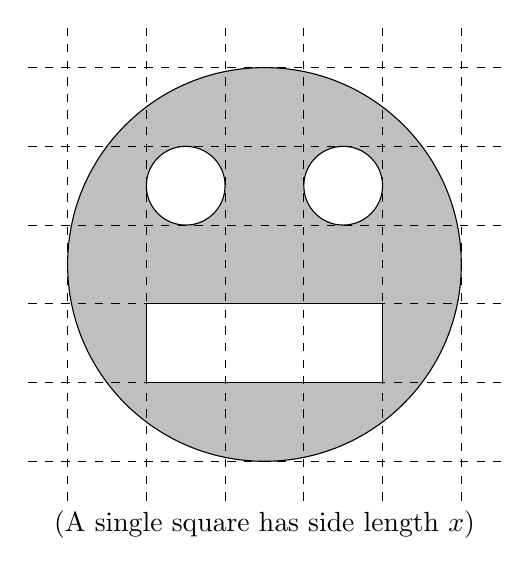
\begin{tikzpicture}
\filldraw[fill=black!25] (3.5,2.5) circle[radius=2.5];
\filldraw[fill=white] (2.5,3.5) circle[radius=0.5];
\filldraw[fill=white] (4.5,3.5) circle[radius=0.5];
\filldraw[fill=white] (2,1) rectangle ++ (3,1);
\draw[dashed] (0.5,-0.5) grid (6.5,5.5);
\node at (current bounding box.south) [below] {(A single square has side length $x$)};
\end{tikzpicture}
}
\par\ifttm\else\penalty+10000\fi
A figure an squared paper.
\end{center}
%%\fi

Answer:
\begin{itemize}
\item{The large circle has in total an area of \MLFunctionQuestion{25}{25/4*pi*x*x}{5}{x}{5}{ERX11},}
\item{each smaller circle has an area of \MLFunctionQuestion{25}{1/4*pi*x*x}{5}{x}{5}{ERX12},}
\item{the area of the figure is in total \MLFunctionQuestion{40}{(25/4*pi-1/2*pi-3)*x*x}{5}{x}{5}{ERX13}.}
\end{itemize}
\MInputHint{The number $\pi$ can be entered as \texttt{pi}.}

\begin{MHint}{Hint for calculating the area}
The calculation of areas is presented in later chapters. To solve this exercise you only need to know, that
a rectangle of side lengths $a$ and $b$ has the area $a\cdot b$ (entered as \texttt{a*b}) and  
a circle of radius $r$ has the area $\pi r^2$ (entered as \texttt{pi*r\^2}).
\end{MHint}

\begin{MHint}{Solution}
The large circle has in total the area $\Mtfrac{25}{4}\pi x^2$ (entered as \texttt{25/4*pi*x*x}).
Each smaller circle has the area $\Mtfrac{1}{4}\pi x^2$, and the whole figure has the area 
$(\Mtfrac{25}{4}\pi-\Mtfrac{1}{2}\pi-3)\cdot x^2$.
\end{MHint}
\end{MExercise}

\end{MXContent}

\begin{MXContent}{Transformation of terms}{Transformation of terms}{STD}
\MLabel{VBKM01_TermeUmformen}
\MDeclareSiteUXID{VBKM01_TermeUmformen}
Different operations in a term can express the same value. For example, $x+x$ is a different 
arrangement of symbols than $2x$, but describes the same term, i.e. if $x$ is substituted with a specific number, then 
$x+x$ and $2x$ provide the same value.

\begin{MInfo}
Terms are related by an equals sign if they are always evaluated to the same value.
\end{MInfo}

In general, new terms are created by transformation of existing terms:

\begin{MInfo}
A \MEntry{transformation}{transformation} of a term is created by applying one or more calculation 
rules to the term:

\begin{itemize}
\item{Collecting: $a+a+\cdots+a=n\cdot a$ ($n$ is the number of addends).}
\item{Distributive property  (``expansion''): $(a+b)\cdot c = a c+b c$ and $c\cdot(a+b)=c a+c b$.}
\item{Commutative property: $a+b=b+a$.}
\item{Associative property (``group numbers differently in operations of the same kind''): \\$a+(b+c)=(a+b)+c=a+b+c$, 
also possible in multiplications.}
\item{Calculation rules for powers and special functions.}
\item{Calculation rules for specific types of terms (e.g.\ the binomial formulas).}
\item{Calculation rules for fractions: $\Mtfrac1{\phantom{2}\Mtfrac{a}{b}\phantom{2}}=\Mtfrac{b}{a}$.}
\end{itemize}
\end{MInfo}

The rules will be presented in detail in the following sections. Often, the aim of this transformation is to 
simplify the term, to isolate individual variables, or to transform a term into a required form:


\begin{MExample}
Allowed transformations are:
\begin{itemize}
\item{$a(a+a+a)+a^2+a^2+a^2 = 6a^2$: the term on the right is simpler, since it requires less symbols.}
\item{$(x+3)^2-9=x^2+6x$ (first binomial formula): both terms describe a parabola. On the left, 
the vertex $(-3,-9)$ of the parabola can be seen easily, on the right, the two roots ($x_1=0$ and $x_2=-6$)
can be seen easily.}
\item{$1+3x+3x^2+x^3=(1+x)^3$: on the right, it can be seen, for example, that the function described by the 
term has only the root $x_1=-1$.}
\item{$\Mtfrac{a+1}{a}=1+\Mtfrac{1}{a}$: on the left, it can be seen, that the term has the root $a_1=-1$, 
on the right it can be seen, that, for very large $a$, the term converges to $1$ (since $\Mtfrac{1}{a}$ is very 
small in this case).}
\end{itemize}
\end{MExample}


\begin{MExerciseCollection}{TESTCOLLECTION001}{1}

\begin{MExercise}
Transform into a sum: \MEquationItem{$a\cdot(b+c)+c\cdot(a+b)$}{\MLSimplifyQuestion{20}{a*(b+c)+c*(a+b)}{3}{a,b,c}{3}{1}{TC1}}.
\begin{MHint}{Solution}
$$
a\cdot(b+c)+c\cdot(a+b) \;=\; a b + a c + c a + c b \;=\; a b + 2 a c + b c
$$
\end{MHint}
\end{MExercise}
\newpage

\begin{MExercise}
Transform into a sum: \MEquationItem{$(x-y)(z-x)+(x-z)(y-z)$}{\MLSimplifyQuestion{20}{(x-y)*(z-x)+(x-z)*(y-z)}{3}{x,y,z}{3}{1}{TC2}}.
\begin{MHint}{Solution}
$$
(x-y)(z-x)+(x-z)(y-z) \;=\; x z - x^2 -y z +y x + x y - x z - z y + z^2 \;=\; -x^2 - 2 y z + 2 x z + z^2
$$
\end{MHint}
\end{MExercise}

\begin{MExercise}
Transform into a sum: \MEquationItem{$(a+b+2)(a+1)$}{\MLSimplifyQuestion{20}{(a+b+2)*(a+1)}{3}{a,b,c}{3}{1}{TC3}}.
\begin{MHint}{Solution}
$$
(a+b+2)(a+1) \;=\; a^2 + b a + 2a + a + b + 2 \;=\; a^2 + a b + 3a + b +2
$$
\end{MHint}
\end{MExercise}

\end{MExerciseCollection}




\end{MXContent}


\MSubsection{Fractional Arithmetic}
\MLabel{M01_Bruchrechnung}
\begin{MXContent}{Calculating with Fractions}{Calculating with Fractions}{STD}
\MDeclareSiteUXID{VBKM01_Bruchrechnung}

A fraction is a rational number of the form $\displaystyle \Mtfrac{\mbox{numerator}}{\mbox{denominator}}$,
where numerator and denominator are integers, and the denominator holds $\neq 0$. Examples are:
$$\Mdfrac{1}{2}\MDFPSpace, \MDFPaSpace\Mdfrac{5}{-10}\MDFPSpace, \MDFPaSpace\Mdfrac{-17}{12}\MDFPSpace, 
\MDFPaSpace\Mdfrac{1}{23}\MDFPSpace, \MDFPaSpace\Mdfrac{4}{6}\MDFPSpace, \MDFPaSpace\Mdfrac{-2}{3}\MDFPSpace, 
\MDFPaSpace \ldots \MDFPeriod$$
It can be seen very quickly, that one and the same number can have an arbitrary number of equivalent 
representations. For example, it holds:
$$\Mdfrac{12}{36} = \Mdfrac{1}{3} = \Mdfrac{24}{72} = \Mdfrac{-12}{-36} = \Mdfrac{3}{9} = \Mdfrac{2}{6} = \Mdfrac{120}{360}= \dots \MDFPeriod$$
The different representations transform into each other by \textbf{reducing} and \textbf{expanding}, respectively.
\begin{MInfo}
Fractions are \MEntry{reduced}{reducing} by dividing numerator and denominator by 
the same non-zero integer.

Fractions are \MEntry{expanded}{expanding} by multiplying numerator and denominator by 
the same non-zero integer.
\end{MInfo}

\begin{MExample}
Three friends like to share a pizza. Tom eats $\displaystyle \Mtfrac{1}{4}$ of the pizza, Tim eats
$\displaystyle \Mtfrac{1}{3}$ of the pizza. How much of the pizza is left for their friend Sven, 
who always has the biggest appetite?\\
The solution is found by means of fractional arithmetic: At first, we have to add 
two fractions to decide, how much of the pizza Tim and Tom already ate:
$$\Mdfrac{1}{4} + \Mdfrac{1}{3} = \Mdfrac{1\cdot 3}{4\cdot 3}+\Mdfrac{1\cdot 4}{3\cdot 4} 
= \Mdfrac{3}{12} +\Mdfrac{4}{12} = \Mdfrac{7}{12} \MDFPeriod$$
Here, we can already identify the two most important steps: 
At first, we have to expand the two fractions to the so called 
\textbf{least common denominator}, or, as one also says, we have to create
\textbf{like} fractions. Then, if the fractions have the same denominator, 
we can add them by adding their numerators and maintaining the denominator. 
>From the result, that Tim and Tom ate 
$\displaystyle \Mtfrac{7}{12}$ of the pizza, we can calculate
how much of the pizza is left for Sven by subtracting 
$\displaystyle \Mtfrac{7}{12}$ from 1:
$$ 1 - \Mdfrac{7}{12} = \Mdfrac{12}{12} - \Mdfrac{7}{12} = \Mdfrac{5}{12} \MDFPeriod$$
Again, we have to expand the fractions to the least common 
denominator. Then we have to subtract the two numerators. Indeed, the two friends
have left much of the pizza for the always hungry Sven.
\end{MExample}

In the following training exercise the reducing of fractions can be practised.

\MDirectRouletteExercises{fraction_cancellation.rtex}{VBKM01_FRACTIONTRAINING}
\newpage

It becomes more difficult, if indeterminate expressions (e.g.\ variables) occur in 
numerator and denominator. These can be reduced or cancelled just like numbers (but not 
with numbers), for example,
$$
\frac{4x^2y^3+3y^2}{10y^2} \;=\; \frac{4x^2y+3}{10}
$$
by cancelling the term $y^2$ from numerator and denominator. The following training exercise
has been extended to fractions including indeterminate expressions.

\MDirectRouletteExercises{vfraction_cancellation.rtex}{VBKM01_VFRACTIONTRAINING}


\begin{MInfo}
The \MEntry{least common denominator}{least common denominator} of two fractions
is the least common multiple (lcm) of the two denominators.

The \MEntry{least common multiple}{lcm} (lcm) of two numbers is the smallest number that 
is divisible by both numbers.

The \MEntry{greatest common divisor}{gcd} (gcd) of two numbers is the largest number that
divides both numbers without remainder.
\end{MInfo}

In case the determination of the lcm is too complicated, also the 
simple product of the denominators can be used instead of the lcm in the following 
calculation rule:


\begin{MInfo}
Fractions are \MEntry{added/subtracted}{adding (fractions)} by finding
a common denominator and then adding/substrac\-ting the numerators, i.e.
$$\Mdfrac{a}{b} \pm \Mdfrac{c}{d} = \Mdfrac{a d\pm b c}{b d} \MDFPSpace, \MDFPaSpace b d\neq 0 \MDFPeriod$$
Usually fractions are expanded to the least common denominator.
\end{MInfo}

For example, the least common multiple of $6=2\cdot 3$ and $15=3\cdot 5$ is the number 
$2\cdot3\cdot 5=30$. However, the product is $6\cdot 15=90$. Thus, you can calculate
$$
\Mdfrac{1}{6}+\Mdfrac{1}{15} \;=\; \Mdfrac{5}{30}+\Mdfrac{2}{30} \;=\; \Mdfrac{7}{30}
$$
but also
$$
\Mdfrac{1}{6}+\Mdfrac1{15} \;=\; \Mdfrac{15}{90}+\Mdfrac{6}{90} \;=\; \Mdfrac{21}{90}
$$
and finally reduce the last fraction to $\Mtfrac{7}{30}$.

\begin{MExample}
The least common multiple for the least common denominator is the smallest number that can
be divided by all denominators involved. If these denominators have no factors in common, the 
least common multiple is simply the product of all denominators:
\begin{eqnarray*}
\Mdfrac{1}{6}+\Mdfrac{1}{10} &=& \Mdfrac{5}{30}+\Mdfrac{3}{30} \;=\; \Mdfrac{8}{30} \;=\; \Mdfrac{4}{15}\MDFPSpace , \ \\
\Mdfrac{1}{6}+\Mdfrac{1}{10} &=& \Mdfrac{10}{60}+\Mdfrac{6}{60} \;=\; \Mdfrac{16}{60} \;=\; 
\Mdfrac{4}{15}\MDFPaSpace  \text{(also correct)}, \ \\
\Mdfrac{4}{15}-\Mdfrac1{2} &=& \Mdfrac{8}{30}-\Mdfrac{15}{30} \;=\; \Mdfrac{8-15}{30} \;=\; -\Mdfrac{7}{30}\MDFPSpace , \ \\
\Mdfrac{1}{3}+\Mdfrac{1}{9} &=& \Mdfrac{3}{9}+\Mdfrac19 \;=\; \Mdfrac49\MDFPSpace ,\ \\
\Mdfrac1{2^2}+\Mdfrac1{2^4} & = & \Mdfrac{2^2}{2^4}+\Mdfrac{1}{2^4} \;=\; \Mdfrac{5}{16}\MDFPSpace ,\ \\
\Mdfrac12+\Mdfrac13+\Mdfrac17 & = & \Mdfrac{21}{42}+\Mdfrac{14}{42}+\Mdfrac{6}{42} \;=\; \Mdfrac{41}{42}\MDFPeriod
\end{eqnarray*}
\end{MExample}

The least common denominator can be also found if the denominators include variables. Since
the transformations of the fractions have to be correct for all possible values of these variables, 
they have to be considered as numbers without any common factors:

\begin{MExample}
Let $x$ and $y$ be variables, then
\begin{eqnarray*}
\Mdfrac13+\Mdfrac1x & = & \Mdfrac{x}{3\cdot x}+\Mdfrac{3}{3\cdot x} \; =\; \Mdfrac{3+x}{3\cdot x}\MDFPSpace ,\\
\Mdfrac{1}{x}+\Mdfrac1{y} & = & \Mdfrac{y}{x\cdot y}+\Mdfrac{x}{x\cdot y} \;=\; \Mdfrac{x+y}{x\cdot y}\MDFPSpace ,\ \\
\Mdfrac{1}{(x+1)^2}+\Mdfrac1{x+1} & = & \Mdfrac{1}{(x+1)^2}+\Mdfrac{x+1}{(x+1)^2}\;=\;\Mdfrac{x+2}{(x+1)^2}\MDFPeriod
\end{eqnarray*}
\end{MExample}

\begin{MExercise}
Calculate the following sums by means of the least common denominator 
(or the product of the denominators).
\begin{MExerciseItems}
\item{\MEquationItem{$\Mtfrac12-\Mtfrac18$}{\MLSimplifyQuestion{20}{-1/8+1/2}{4}{}{4}{16}{HN1}}.}
\item{\MEquationItem{$\Mtfrac13+\Mtfrac15+\Mtfrac16$}{\MLSimplifyQuestion{20}{1/3+1/5+1/6}{4}{}{4}{16}{HN2}}.}
\item{\MEquationItem{$\Mtfrac1{2x}+\Mtfrac1{3x}$}{\MLSimplifyQuestion{20}{5/(6*x)}{4}{x}{4}{528}{HN3}}.}
\end{MExerciseItems}
\MInputHint{Please use no other operators than the operators for multiplication \texttt{*} 
and division \texttt{/} during this exercise.}

\begin{MHint}{Solution}
Finding the least common denominator and collecting/reducing gives
\begin{eqnarray*}
\Mdfrac12-\Mdfrac18 & = & \Mdfrac48-\Mdfrac18 \;=\; \Mdfrac38 \MDFPSpace ,\\
\Mdfrac13+\Mdfrac15+\Mdfrac16 & = & \Mdfrac{10}{30}+\Mdfrac6{30}+\Mdfrac{5}{30} \;=\; \Mdfrac{21}{30} \;=\; \Mdfrac{7}{10}\MDFPSpace ,\\
\Mdfrac1{2x}+\Mdfrac1{3x} & = & \Mdfrac{3}{6x}+\Mdfrac{2}{6x} \;=\; \Mdfrac{5}{6x} \MDFPSpace .
\end{eqnarray*}
\end{MHint}
\end{MExercise}

\begin{MExercise}
In the case of like fractions, you may only add or decompose the nominators, 
for denominators no such rule exists. To convince yourself, calculate the following numbers
by finding the least common denominator and reducing 
as much as possible:
\begin{MExerciseItems}
\item{\MEquationItem{$\Mdfrac12+\Mdfrac13$}{\MLSpecialQuestion{10}{5/6}{5}{0}{0}{exactfraction}{GLN1}} but \MEquationItem{$\Mdfrac1{2+3}$}{\MLSpecialQuestion{12}{1/5}{5}{0}{0}{exactfraction}{GLN2}}.}
\item{\MEquationItem{$\Mdfrac{1+2}{5+6}$}{\MLSpecialQuestion{12}{3/11}{5}{0}{0}{exactfraction}{GLN3}} but \MEquationItem{$\Mdfrac15+\Mdfrac26$}{\MLSpecialQuestion{12}{8/15}{5}{0}{0}{exactfraction}{GLN4}}.}
\end{MExerciseItems}
\begin{MHint}{Solution}
Sums of denominators may not be collected, not even in the case of like nominators. Here is
$$
\Mdfrac12+\Mdfrac13\;=\; \Mdfrac{3}{6}+\Mdfrac26 \;=\; \Mdfrac56\;\;\text{but}\;\;
\Mdfrac{1}{2+3} \;=\; \Mdfrac15\MDFPSpace .
$$
Also, the simple ``splitting'' of fraction parts is not allowed, here is
$$
\Mdfrac{1+2}{5+6} \;=\; \Mdfrac{3}{11}  \;\;\text{but}\;\; \Mdfrac15+\Mdfrac26 \;=\; \Mdfrac{6}{30}+\Mdfrac{10}{30} \;=\; \Mdfrac{16}{30}\;=\; \Mdfrac{8}{15}\MDFPSpace .
$$
\end{MHint}
\end{MExercise}

\begin{MInfo}
Two fractions are \MEntry{multiplied}{multiplication (fractions)} by multiplying the 
numerators and multiplying the denominators, i.e.\
$$\Mdfrac{a}{b} \cdot \Mdfrac{c}{d} = \Mdfrac{a\cdot c}{b\cdot d}\MDFPSpace, \MDFPaSpace b d\neq 0 \MDFPeriod$$
\end{MInfo}

The division of two fractions is reduced to their multiplication:

\begin{MInfo}
Two fractions are \MEntry{divided}{division (fractions)} by multiplying the first fraction with the reciprocal of 
the second fraction, i.e. 
$$\Mdfrac{a}{b} : \Mdfrac{c}{d} = \Mdfrac{a}{b} \cdot \Mdfrac{d}{c} = \Mdfrac{a\cdot d}{b\cdot c}\MDFPSpace, \MDFPaSpace b,c,d\neq 0 \MDFPeriod$$
The division of two fractions can be expressed as a \textbf{compound fraction} as well:
$$\Mdfrac{a}{b} : \Mdfrac{c}{d} = \Mdfrac{\Mdfrac{a}{b}}{\Mdfrac{c}{d}} \MDFPeriod$$
\end{MInfo}

\begin{MExample}
Taking possible reducing into account, the multiplication and the division of two fractions, respectively, 
takes the following form:
$$\Mdfrac23\cdot \Mdfrac45 = \Mdfrac{2\cdot 4}{3\cdot 5} = \Mdfrac{8}{15}\MDFPSpace, \MDFPaSpace \Mdfrac23 : \Mdfrac45 = \Mdfrac23\cdot \Mdfrac54 = \Mdfrac{10}{12} = \Mdfrac56 \MDFPeriod$$
\end{MExample}


\end{MXContent}

\begin{MXContent}{Converting Fractions}{Converting Fractions}{STD}
\MDeclareSiteUXID{VBKM01_USBrueche}
Dividing the denominator into the numerator gives a \MEntry{decimal fraction}{decimal fraction} or 
a decimal number, respectively, for example,
$$\Mdfrac{1}{2} = \MZahl{0}{5} \MDFPSpace, \MDFPaSpace \Mdfrac{1}{3} = \MZahl{0}{33333}\ldots= \MZahl{0}{}\bar{3} \MDFPSpace, \MDFPaSpace \Mdfrac{1}{7} = \MZahl{0}{}\overline{142857} \MDFPSpace, \MDFPaSpace \Mdfrac{1}{8} = \MZahl{0}{125} \MDFPeriod$$
By means of these examples it can already be seen, that the division is either finite, leading to a
\MEntry{proper decimal fraction}{decimal fraction (proper)}, or the digits of the decimal number repeat in a 
certain way, leading to an \MEntry{infinite repeating decimal fraction}{decimal fraction (repeating)}.

Converting decimal numbers to fractions is done using the base-10 positional notation. Each 
decimal number has the form
\begin{center}
\ifttm\else\dots\fi\,\begin{tabular}{|c|c|c|c|c|c|c|c|c|c|}
\hline
1&2&3&4&5&\MZXYZhltrennzeichen &6&7&8&9\\
\hline
TTH&TH&H&T&O&\MZXYZhltrennzeichen 
&t&h&th&tth\\
\hline
\end{tabular}\,\ifttm\else\dots\fi
\end{center}
\vspace*{5mm}

with the abbreviations TTH \ldots\ ten thousands, TH \ldots\ thousands, 
H \ldots\ hundreds, T \ldots\ tens, O \ldots\ ones, t \ldots\ tenths, 
h \ldots\ hundredths, th \ldots\ thousandths, tth \ldots\ 
ten thousandths etc.\\
Then, the conversion is done as follows:
\begin{eqnarray*}
\MZahl{4}{375} &=& 4 + \Mdfrac{3}{10}+\Mdfrac{7}{100}+\Mdfrac{5}{1000} \ \\
&=& 4 + \Mdfrac{300+70+5}{1000} \ \\
&=& 4 + \Mdfrac{375}{1000}\ \\
&=& 4 + \Mdfrac{75}{200} \ \\
&=& 4 + \Mdfrac{15}{40} = \Mdfrac{35}{8} \MDFPeriod
\end{eqnarray*}
But what about converting an infinite repeating decimal number? It seems that we would have to
add an infinite number of fractions, which is in practise of less use, of course. Therefore, in
\textbf{converting infinite repeating decimal numbers to fractions} we use a trick:

\begin{MInfo}
\MLabel{Mathematik_Grundlagen_UDB}
\MEntry{Converting}{converting (decimal fractions)} infinite repeating decimal numbers to fractions is 
done by multiplying the decimal number with a power of ten such that the repeating digits are shifted 
to the left of the decimal point. This leads to an equation of the form $10^k\cdot x=x+n$ for the decimal 
number $x$, that can be solved for $x$: $x=\Mdfrac{n}{10^k-1}$ (which is a simple fraction).
\end{MInfo}

\begin{MExample}
The number $\MZahl{0}{}\bar 6$ is to be converted to a fraction. For this, you multiply the number by 
$10$ and subtract from the result the initial number to eliminate the infinite repeating decimal:
\begin{center}
\begin{tabular}{crclcr}
	&$10$ & $\cdot$ & $\MZahl{0}{}\bar 6$ & = & $\MZahl{6}{}\bar 6$\\
	$-$ & $1$ & $\cdot$ & $\MZahl{0}{}\bar 6$ & = & $\MZahl{0}{}\bar 6$\\
\hline
$\Rightarrow$&$9$ & $\cdot$ & $\MZahl{0}{}\bar 6$ & = & $\MZahl{6}{0}$\\
\end{tabular}
\end{center}
>From the last relation, it immediately follows after division by $9$:
\quad $\displaystyle \MZahl{0}{}\bar 6 = \Mtfrac{6}{9} = \Mtfrac{2}{3}.$
\end{MExample}

This method also works, if not all digits after the decimal point repeat periodically:

\begin{MExample}
The decimal number $\MZahl{0}{8}\bar{3}=\MZahl{0}{83333}\ldots$ is to be converted to 
a fraction:
\begin{center}
\begin{tabular}{crclcr}
&$100$ & $\cdot$ & $\MZahl{0}{8}\bar 3$ & = & $\MZahl{83}{}\bar 3$\\
$-$&$10$ & $\cdot$ & $\MZahl{0}{8}\bar 3$ & = & $\MZahl{8}{}\bar 3$\\
\hline
$\Rightarrow$&$90$ & $\cdot$ & $\MZahl{0}{8}\bar 3$ & = & $\MZahl{75}{0}$\\
\end{tabular}
\end{center}
Division by $90$ gives the result: $\displaystyle \MZahl{0}{8}\bar 3 = \Mtfrac{75}{90} = \Mtfrac{5}{6}$.
\end{MExample}

Thus, the method is always the same: by multiplying by powers of ten and subsequent 
subtraction the infinite repeating decimal is removed.

\begin{MExercise}
Using the above method, find a simple and fully reduced fraction that represents the
value $\MZahl{0}{45555}\ldots$.
\ \\ \ \\
Answer: \MEquationItem{$\displaystyle \MZahl{0}{4}\overline{5}$}{\MLSpecialQuestion{12}{41/90}{5}{0}{0}{exactfraction}{BRZ3}}.
\ \\
\MInputHint{Enter the fraction as \texttt{numerator/denominator} fully reduced and with 
positive denominator.}
\ \\
\begin{MHint}{Solution}
Multiplying $x=\MZahl{0}{4}\overline{5}$ by an appropriate power of ten gives
$$
10x-x=\MZahl{4}{1}\;\Rightarrow\; 9x=\Mdfrac{41}{10}\;\Rightarrow\;x=\Mdfrac{41}{90} \MDFPeriod
$$
this fraction is already fully reduced as well.
\end{MHint}
\end{MExercise}

However, in \MEntry{back-of-the-envelope calculations}{back-of-the-envelope calculation} 
(i.e. if you only want to roughly estimate the magnitude or the ratio of one number to the other without 
knowing the correct values of the decimal fractions) it is useful to multiply the numbers by the least 
common denominator instead of converting them to decimals:

\begin{MExample}
\MLabel{VBKM01_Bsp_Anordnung}
The fractions $\frac23$, $\frac{32}{12}$, and $\frac{12}{15}$ are to be arranged in order of size.
For this, the fractions are multiplied by the least common denominator ($60$, in this case). 
The denominators are cancelled and the fractions are converted to the integers
$$
\frac23\cdot 60\;=\; 2\cdot 20\;=\; 40 \;\; ,\;\;
\frac{32}{12}\cdot 60 \;=\; 32\cdot 5\;=\; 160 \;\; , \;\;
\frac{12}{15}\cdot 60 \;=\; 12\cdot 4 \;=\; 48 \MDFPeriod
$$
Arrangement in order of size gives $40<48<160$. With this, we have $\frac23<\frac{12}{15}<\frac{32}{12}$, 
since the multiplication of the fractions by the same integer $60$ does not change the arrangement of
the fractions (see section \MNRef{M03_Ungleichungen}, which deals with inequalities and their 
transformation).
\end{MExample}

\begin{MExercise}
Arrange the fractions 
$\frac{16}{15}$, $\frac12$, $\frac23$, $\frac2{-3}$, $\frac{60}{90}$, and $\frac43$ in order of size?
\ \\
\MLParsedQuestion{7}{2/(-3)}{5}{VBKM01_USR1}\ $<$\ 
\MLParsedQuestion{7}{2/3}{5}{VBKM01_USR2}\ $=$\ 
\MLParsedQuestion{7}{60/90}{5}{VBKM01_USR3}\ $<$\ 
\MLParsedQuestion{7}{1/2}{5}{VBKM01_USR4}\ $<$\ 
\MLParsedQuestion{7}{16/15}{5}{VBKM01_USR5} \ $<$\ 
\MLParsedQuestion{7}{4/3}{5}{VBKM01_USR6} .
\ \\
\begin{MHint}{Solution}
Multiplying by the common denominator $180$ gives the numbers $90$, $60$, $-60$, $270$, and $60$,
which leads to the arrangement
$$
-60\; < \; 60 \; = \; 60 \; < \; 90\; < \; 96 \; < \; 120
$$
and thus finally to 
$$
\frac2{-3} \; < \; \frac23 \;=\; \frac{60}{90} \; <\; \frac12\; < \; \frac{16}{15} \; < \; \frac{4}{3}.
$$
\end{MHint}
\end{MExercise}

\end{MXContent}

\begin{MExercises}
\MDeclareSiteUXID{VBKM01_Bruchrechnung_Exercises}

\begin{MExercise}
Reduce the following fractions to the lowest terms:

\begin{MExerciseItems}
\item{\MEquationItem{$\displaystyle \Mdfrac{216}{240}$}{\MLSpecialQuestion{8}{9/10}{5}{0}{0}{exactfraction}{BRF1}}. \begin{MHint}{Solution}Since $\MGGT(216,240)=24$ we have $\displaystyle\Mdfrac{216}{240}=\Mdfrac{216:24}{240:24}=\Mdfrac{9}{10}$.\end{MHint}}
\item{\MEquationItem{$\displaystyle \Mdfrac{36}{72}$}{\MLSpecialQuestion{8}{1/2}{5}{0}{0}{exactfraction}{BRF2}}. \begin{MHint}{Solution}$36$ divides $72$, hence $\Mdfrac{36}{72}=\Mdfrac{1}{2}.$\end{MHint}} 
\item{\MEquationItem{$\displaystyle \Mdfrac{48}{144}$}{\MLSpecialQuestion{8}{1/3}{5}{0}{0}{exactfraction}{BRF3}}. \begin{MHint}{Solution}$48$ divides $144$, hence $\Mdfrac{48}{144}=\Mdfrac{1}{3}.$\end{MHint}}
\item{\MEquationItem{$\displaystyle\Mdfrac{-a+2b}{-4b+2a}$}{\MLSpecialQuestion{8}{-1/2}{5}{0}{0}{exactfraction}{BRF4}} if $a$ not equals \MLSimplifyQuestion{5}{2*b}{5}{a,b}{5}{1}{BRF4b}. \begin{MHint}{Solution}Reducing gives $\Mdfrac{-a+2b}{-4b+2a}=\Mdfrac{(-1)\cdot (-2b+a)}{2\cdot (-2b+a)}=-\Mdfrac12$. The fraction is only defined for $a\not=2b$.\end{MHint}} 
%\item $\displaystyle\Mdfrac{18\cdot u^2\cdot v \cdot w^3}{45\cdot u\cdot v\cdot w^2}$, \quad $u,v,w\neq 0$\\\begin{MHint}{Solution} $$\Mdfrac{18\cdot u^2 \cdot v\cdot w^3}{45\cdot u\cdot v\cdot w^2}=\Mdfrac{2\cdot u\cdot w}{5}$$\end{MHint} 
\end{MExerciseItems}
\MInputHint{Enter the fraction as \texttt{numerator/denominator} fully reduced and with 
positive denominator. Always place the signs in front of the fractions, and do not use  
brackets.}
\end{MExercise}

% \begin{MExercise}
% Eine wichtige Anwendung der Bruchrechnung findet sich in der Musik. 
% \begin{enumerate}
% \item Stellen Sie fest, um welche Takte es sich hierbei handelt, wenn die folgenden Noten in einem Takt gegeben sind:
% 
% \textbf{a)} $\displaystyle \Mdfrac18, \Mdfrac18, \Mdfrac12$ \qquad \textbf{b)} $\displaystyle \Mdfrac{1}{16}, \Mdfrac14, \Mdfrac{1}{16}, \Mdfrac14, \Mdfrac18$ \qquad \textbf{c)} $\displaystyle \Mdfrac18, \Mdfrac{1}{16}, \Mdfrac14, \Mdfrac{1}{16}$
% \ \\
% \begin{MHint}{Solution}
% Die Summe der Notenl"angen zeigt an, wieviele ganze Noten ein Takt besitzt:
% \begin{itemize}
% \item{$\displaystyle \Mdfrac18+\Mdfrac18+\Mdfrac12=\Mdfrac{1+1+4}{8}=\Mdfrac68$ oder $\displaystyle \Mdfrac34$,}
% \item{$\displaystyle \Mdfrac{1}{16}+ \Mdfrac14+ \Mdfrac{1}{16}+ \Mdfrac14+ \Mdfrac18=\Mdfrac{1+4+1+4+2}{16}=\Mdfrac{12}{16}=\Mdfrac{6}{8}$ oder $\displaystyle \Mdfrac34$,}
% \item{$\displaystyle \Mdfrac18+ \Mdfrac{1}{16}+ \Mdfrac14+ \Mdfrac{1}{16}=\Mdfrac{2+1+4+1}{16}=\Mdfrac{8}{16}=\Mdfrac12$ oder $\displaystyle \Mdfrac24$.}
% \end{itemize}
% \end{MHint}
% \ \\
% \item Welche Noten fehlen, damit es sich um einen $\displaystyle \Mdfrac34$-Takt handelt?
% \ \\
% \textbf{a)} $\displaystyle \Mdfrac18, \Mdfrac14$ \qquad \textbf{b)} $\displaystyle \Mdfrac{1}{16}, \Mdfrac18, \Mdfrac18$
% \ \\
% \begin{MHint}{Solution}
% Wir erg"anzen die Summe der Noten zum Bruch $\Mdfrac34$:
% \begin{itemize}
% \item{$\displaystyle \Mdfrac18+ \Mdfrac14=\Mdfrac38$, addiert man drei Achtelnoten, so erh"alt man $\displaystyle \Mdfrac38+\Mdfrac38=\Mdfrac68=\Mdfrac34$,}
% \item{$\displaystyle \Mdfrac{1}{16}+ \Mdfrac18+ \Mdfrac18=\Mdfrac{5}{16}$, addiert man 7 Sechzehntelnoten (oder eine andere Aufteilung die zu $\displaystyle \Mdfrac7{16}$ in der Summe f"uhrt), so ist die Gesamtsumme $\displaystyle \Mdfrac5{16}+\Mdfrac7{16}=\Mdfrac{12}{16}=\Mdfrac34$.}
% \end{itemize}
% \end{MHint}
% \end{enumerate} 
% 
% \end{MExercise}

\begin{MExercise}
Calculate and fully reduce the following expressions for appropriate numbers $a,b,x,y$:
\begin{MExerciseItems}
\item{\MEquationItem{$\displaystyle \Mdfrac12-\Mdfrac27+\Mdfrac38+\Mdfrac34$}{\MLSpecialQuestion{10}{75/56}{5}{0}{0}{exactfraction}{BRX1}}. \begin{MHint}{Solution}Adding up the numerators over the least common denominator gives $\Mdfrac12-\Mdfrac27+\Mdfrac38+\Mdfrac34=\Mdfrac{28}{56}-\Mdfrac{16}{56}+\Mdfrac{21}{56}+\Mdfrac{42}{56}=\Mdfrac{75}{56}$, since $\MGGT(2,7,8,4)=56$.\end{MHint}}
\item{\MEquationItem{$\displaystyle \Mdfrac{3}{13}:\Mdfrac{7}{26}$}{\MLSpecialQuestion{10}{6/7}{5}{0}{0}{exactfraction}{BRX2}}. \begin{MHint}{Solution}Dividing by a fraction is the same as multiplying by its reciprocal: $\Mdfrac{3}{13}:\Mdfrac{7}{26}=\Mdfrac{3}{13}\cdot\Mdfrac{26}{7}=\Mdfrac{3\cdot 26}{13\cdot 7}=\Mdfrac{3\cdot 2}{1\cdot 7}=\Mdfrac67$.\end{MHint}}
\item{\MEquationItem{$\displaystyle \left(\MZahl{1}{}\bar{4}\cdot 3-\Mdfrac12\right)\cdot\Mdfrac{6}{7}$}{\MLSpecialQuestion{10}{23/7}{5}{0}{0}{exactfraction}{BRX3}}. \begin{MHint}{Solution}Converting the decimal expression to a fraction gives 
$\left(\MZahl{1}{}\bar{4}\cdot 3-\Mdfrac12\right)\cdot\Mdfrac{6}{7}=\left(\MZahl{1}{}\bar{4}\cdot 18-3\right)\cdot\Mdfrac{1}{7}=\left(26-3\right)\cdot\Mdfrac{1}{7}=\Mdfrac{23}{7}$.\end{MHint}}
%%\item{\MEquationItem{$\displaystyle \Mdfrac{3a}{3a+6b}+\Mdfrac{2b}{a+2b}$}{\MLSpecialQuestion{10}{1}{5}{0}{0}{exactfraction}{BRX4}}. \begin{MHint}{Solution}Summieren über den Hauptnenner ergibt
%%$\Mdfrac{3a}{3a+6b}+\Mdfrac{2b}{a+2b}=\Mdfrac{3a}{3a+6b}+\Mdfrac{6b}{3a+6b}=\Mdfrac{3a+6b}{3a+6b}=1$.\end{MHint}}
%%\item{\MEquationItem{$\displaystyle \Mdfrac{18x^2-48x y+32y^2}{12y-9x}\cdot \Mdfrac{18x+24y}{9x^2-16y^2}$}{\MLSpecialQuestion{10}{-4}{5}{0}{0}{exactfraction}{BRX5}}. \begin{MHint}{Solution}Vereinfachen des Ausdrucks ergibt
%%\begin{eqnarray*}
%%\Mdfrac{18x^2-48x y+32y^2}{12y-9x}\cdot \Mdfrac{18x+24y}{9x^2-16y^2} & =&
%%4\cdot \Mdfrac{9x^2-24x y+16y^2}{4y-3x}\cdot \Mdfrac{3x+4y}{9x^2-16y^2}\\
%%& =& 4\cdot \Mdfrac{(3x-4y)^2}{4y-3x}\cdot \Mdfrac{3x+4y}{9x^2-16y^2}\\
%%& =& -4\cdot \Mdfrac{(3x-4y)^2}{3x-4y}\cdot \Mdfrac{3x+4y}{(3x+4y)(3x-4y)}=-4 \MDFPeriod
%%\end{eqnarray*}\end{MHint}}
\end{MExerciseItems}
\MInputHint{Enter the fractions fully reduced and with positive numerator.}
\end{MExercise}

\begin{MExercise}
Convert the following infinite repeating decimal fractions to fractions and fully reduce them:
\begin{MExerciseItems}
\item{\MEquationItem{$\displaystyle \MZahl{0}{}\overline{4}$}{\MLSpecialQuestion{12}{4/9}{5}{0}{0}{exactfraction}{BRZ1}}.}
\item{\MEquationItem{$\displaystyle \MZahl{0}{}\overline{23}$}{\MLSpecialQuestion{12}{23/99}{5}{0}{0}{exactfraction}{BRZ2}}.}
\item{\MEquationItem{$\displaystyle \MZahl{0}{12}\overline{34}$}{\MLSpecialQuestion{12}{1222/9900}{9}{0}{0}{exactfraction}{BRZ4}}.}
\item{\MEquationItem{$\displaystyle \MZahl{0}{}\overline{9}$}{\MLSpecialQuestion{12}{1}{5}{0}{0}{exactfraction}{BRZ5}}.}
\end{MExerciseItems}
\MInputHint{Enter the fractions fully reduced and with positive numerator.}
\end{MExercise}
\ \\
\begin{MHint}{Solution}
Using the \MSRef{Mathematik_Grundlagen_UDB}{trick for converting} infinite repeating decimal numbers one gets the following solutions:
\begin{itemize}
\item{$x=\MZahl{0}{}\overline{4}$, hence $\displaystyle 10x-x=4\;\Rightarrow\;9x=4\;\Rightarrow\;x=\Mtfrac49$,}
\item{$x=\MZahl{0}{}\overline{23}$, hence $\displaystyle 100x-x=23\;\Rightarrow\;99x=23\;\Rightarrow\; x=\Mtfrac{23}{99}$,}
\item{$x=\MZahl{0}{12}\overline{34}$, hence $\displaystyle 100x-x=\MZahl{12}{22}\;\Rightarrow\;99x=\Mtfrac{1222}{100}\;\Rightarrow\;x=\Mtfrac{1222}{9900}=\Mtfrac{611}{4950}$,}
\item{$x=\MZahl{0}{}\overline{9}$, hence $\displaystyle 10x-x=9\;\Rightarrow\;9x=9\;\Rightarrow\;x=1$.}
 \end{itemize}
 Note for the last part of this exercise, that $1=\MZahl{1}{000}\ldots$ and $1=\MZahl{0}{999}\ldots=\MZahl{0}{}\overline{9}$
are two decimal representations of one and the same number.
\end{MHint}
\end{MExercises}

\MSubsection{Transformation of terms}
\MLabel{M01_Umformen}


\begin{MIntro}
\MDeclareSiteUXID{VBKM01_UmformenIntro}
What exactly are terms? 
\begin{MInfo}
\MEntry{Terms}{terms} are arithmetic expressions that are combinations of numbers, variables, 
brackets, and appropriate arithmetic operations.
\end{MInfo}

Terms can be interpreted in two ways:
\begin{itemize}
\item{As functional expressions: If each variable contained in the term is substituted with a specific number, 
the term can be evaluated to a certain value. For example, $x+x-1$ is a term; once $x=2$ is inserted one gets the value $3$. The
expression $2x-1$ is a term as well, this term can be transformed into $x+x-1$, and hence it evaluates to the same value if $x=2$ is 
inserted. As a symbolic expression, $x+x-1$ is different from $2x-1$, but as functional expressions they are both the same (equivalent): 
No matter which value is inserted for $x$, both terms are always evaluated to the same value. A term can also be a value for itself, 
if no variables occur. For example, $3\cdot (2+4)$ is a term having the value $18$.}
\item{As evaluation rule: A term can be interpreted as a type of instruction how to calculate a new value from given values 
(inserted into the variables). For example, the term $x^2-1$ can be read as 
``square the value of $x$ and subtract one from the result''. This is different from
the term $(x+1)(x-1)$, even if both terms give the same value. The second term describes the evaluation as  
``add one to $x$ and multiply the result with the value, resulting if $x$ is subtracted by one''. The two terms are 
mathematically equal. One writes $x^2-1=(x-1)(x+1)$, but they represent two different ways for calculating the value. Depending on 
the problem setting, one of the two terms can be more convenient to solve the problem.}
\end{itemize}

\end{MIntro}


\begin{MXContent}{Transformation of Terms}{Transformation of Terms}{STD}
\MDeclareSiteUXID{VBKM01_Termumformungen}

\ \\
Dealing with terms gets interesting, if the equality of two terms is to be investigated or complicated terms are to
be simplified.

\begin{MInfo}\MLabel{Mathematik_Grundlagen_BinomischeFormel}
Two terms are \MEntry{equal}{equality (of terms)}, if they can be transformed into each other by allowed transformations. 
Complicated terms can be simplified using calculation rules. Note in doing so:
\begin{enumerate}
\item Exponentiation precedes multiplication precedes addition.
\item If brackets are involved the distributive property applies:
$$a\cdot(b\pm c) = a\cdot b\pm a\cdot c \MDFPSpace, \MDFPaSpace (a\pm b)\cdot c = a\cdot c \pm b\cdot c \MDFPeriod$$
\item With $d\neq 0$ we have: $\displaystyle (a\pm b):d = \Mtfrac{a}{d}\pm \Mtfrac{b}{d}.$
\item For expressions with nested brackets, first evaluate what's inside the innermost
  set of brackets with respect to the calculation rules and then work your way towards the outermost brackets.
\end{enumerate}
\end{MInfo}

\begin{MExercise}
Remove the brackets from each of the following terms and simplify as far as possible:
\begin{MExerciseItems}
\item{\MEquationItem{$\displaystyle (1-a)\cdot(1-b)$}{\MLSimplifyQuestion{20}{(1-a)*(1-b)}{5}{a,b}{5}{1}{PMPF2}}. \begin{MHint}{Solution}$$(1-a)\cdot(1-b)\;=\; 1-a-b+a b \MDFPeriod $$\end{MHint}}
\item{\MEquationItem{$\displaystyle 5a-(2b-(2a-7b)+4a)-3b$}{\MLSimplifyQuestion{20}{3*a-12*b}{5}{a,b}{5}{1}{PMPF1}}. \begin{MHint}{Solution}$$5a-(2b-(2a-7b)+4a)-3b \; = \; 5a-2b+2a-7b-4a-3b \;=\; 3a-12b \MDFPeriod  $$\end{MHint}}
\end{MExerciseItems}
\MInputHint{The input must not contain any brackets.}
\end{MExercise}

\begin{MInfo}
The three \MEntry{binomial formulas}{binomial formulas} are:
$$ (a+b)^2 = a^2+2a b+b^2 \MDFPSpace, \MDFPaSpace (a-b)^2 = a^2-2a b+b^2 \MDFPSpace,\MDFPaSpace (a+b)(a-b) = a^2-b^2 \MDFPeriod $$
\end{MInfo}

% Exercisen und Fließtext !

Here, for $a$ and $b$ both numbers and whole terms can be inserted.

\begin{MExample}
A few typical applications of the binomial formulas are:
\begin{itemize}
\item{$(1+2x)^2=1^2+2\cdot1\cdot 2x+(2x)^2=1+4x+4x^2$.}
\item{$(1+2x)(1-2x)=1^2-(2x)^2=1-4x^2$.}
\item{$x^4-1=(x^2+1)(x^2-1)=(x^2+1)(x+1)(x-1)$, in this transformation it can be seen, that in the set 
of real numbers $x^4-1$ has only the roots $x=1$ and $x=-1$.}
\item{$(1+x+y)^2=\left({(1+x)+y}\right)^2= (1+x)^2+2(1+x)y+y^2=1+2x+x^2+2y+2x y+y^2$.}
\end{itemize}
\end{MExample}

\begin{MExercise}
Simplify the following term using the second binomial formula:\ \\ \ \\
\MEquationItem{$\displaystyle (-3x+4)(4-3x)$}{\MLSimplifyQuestion{30}{16-24*x+9*x^2}{5}{x}{5}{1}{BMPF4}}.

\begin{MHint}{Solution}$$(-3x+4)(4-3x)\;=\; (4-3x)(4-3x)\;=\; 16-24x+9x^2 \MDFPeriod $$\end{MHint}
\end{MExercise}

\begin{MExample}\MLabel{VBKM01_Bsp_binomial}%
The binomial formulas can be used to transform quadratic expressions cleverly.
This is very useful if squares are to be calculated without any aid. For this, the number to be 
squared is splitted into a simple number (usually a power of ten) and the remainder:
\begin{eqnarray*}
103^2 & = & (100+3)^2 = 100^2+2\cdot 100\cdot 3+3^2 = 10609 \MDFPSpace,\\
49^2 & = & (50-1)^2 = 50^2-2\cdot 50\cdot 1 +1^2 = 2401 \MDFPSpace,\\
61^2-59^2 & = & (61-59)(61+59) = 2\cdot 120 = 240 \MDFPeriod
\end{eqnarray*}
\end{MExample}

\begin{MExercise}%
Using the method described in Example~\MRef{VBKM01_Bsp_binomial}, calculate
\MEquationItem{$\displaystyle 1005^2$}{\MLSimplifyQuestion{8}{1010025}{5}{x}{5}{1024}{BMPF0}}.


\begin{MHint}{Solution}
$$1005^2 \;=\; (1000+5)^2\;=\; 1000000+2\cdot 1000\cdot 5+25 \;=\; 1010025 \MDFPeriod $$\end{MHint}
\end{MExercise}

In the following \MSRef{VBKM01_ExercisenUmformen}{exercise section} you can practise the transformation methods in several exercises.

\end{MXContent}

\begin{MExercises}
\MLabel{VBKM01_ExercisenUmformen}
\MDeclareSiteUXID{VBKM01_Termumformungen_Exercises}
\begin{MExercise}
Simplify the following terms for appropriate numbers $a$, $b$, $x$, $y$, $z$:
\begin{MExerciseItems}
\item{\MEquationItem{$\displaystyle \Mdfrac{3x -6x y^2+4 x y z}{-2x}$}{\MLSimplifyQuestion{20}{-3/2+3*y^2-2*y*z}{5}{x,y,z}{5}{1}{UMPF2}}. \begin{MHint}{Solution}$$\Mdfrac{3x -6x y^2+4 x y z}{-2x}\;=\; -\Mdfrac32+3y^2-2y z \MDFPeriod  $$\end{MHint}}
\item{\MEquationItem{$\displaystyle (3a-2b)\cdot(4a-6)$}{\MLSimplifyQuestion{26}{12*a^2-18*a-8*a*b+12*b}{5}{a,b}{5}{1}{UMPF3}}. \begin{MHint}{Solution} $$(3a-2b)\cdot(4a-6)\;=\; 12a^2-18a-8a b+12b\MDFPeriod  $$\end{MHint}}
\item{\MEquationItem{$\displaystyle (2a+3b)^2-(3a-2b)^2$}{\MLSimplifyQuestion{26}{-5*a^2+24*a*b+5*b^2}{5}{a,b}{5}{1}{UMPF4}}. \begin{MHint}{Solution} \begin{eqnarray*}(2a+3b)^2-(3a-2b)^2&=& (4a^2+12a b+9b^2)-(9a^2-12a b+4b^2)\ \\ &=& -5a^2+24a b+5b^2  \: . \end{eqnarray*}\end{MHint}}
%%\item{\MEquationItem{$\displaystyle \Mdfrac{3a}{3a+6b}+\Mdfrac{2b}{a+2b}$}{\MLSimplifyQuestion{25}{1}{5}{a,b}{5}{1}{UMPF7}}. \begin{MHint}{Solution}$$\Mdfrac{3a}{3a+6b}+\Mdfrac{2b}{a+2b} \; = \; \Mdfrac{a}{a+2b}+\Mdfrac{2b}{a+2b}\;=\; \Mdfrac{a+2b}{a+2b} \;=\; 1 \MDFPeriod $$\end{MHint}}
\item{\MEquationItem{$\displaystyle \Mdfrac{3a}{3a+6b}+\Mdfrac{2b}{a+2b}$}{\MLSpecialQuestion{10}{1}{5}{0}{0}{exactfraction}{UMPF7}}. \begin{MHint}{Solution}Adding up the numerators over the least common denominator gives
$\Mdfrac{3a}{3a+6b}+\Mdfrac{2b}{a+2b}=\Mdfrac{3a}{3a+6b}+\Mdfrac{6b}{3a+6b}=\Mdfrac{3a+6b}{3a+6b}=1$.\end{MHint}}
\end{MExerciseItems}
\MInputHint{The input must not contain any brackets.}
\end{MExercise}

\begin{MExercise}
For the following exercises a little more patience is required. Simplify: \\
\begin{MExerciseItems}
\item{\MEquationItem{$\displaystyle \Mdfrac12x(4x+3y)+\Mdfrac32(5x^2-6x y)$}{\MLSimplifyQuestion{36}{19/2*x^2-15/2*x*y}{5}{x,y}{5}{1}{UMPF5}}. \begin{MHint}{Solution} $$\Mdfrac12x(4x+3y)+\Mdfrac32(5x^2-6x y)\;=\; 2x^2+\Mdfrac32x y+\Mdfrac{15}2x^2-9x y \;=\; \Mdfrac{19}{2}x^2-\Mdfrac{15}{2}x y  \MDFPeriod  $$\end{MHint}}
%%\item{\MEquationItem{$\displaystyle \Mdfrac{18x^2-48x y+32y^2}{12y-9x}\cdot \Mdfrac{18x+24y}{9x^2-16y}$}{\MLSimplifyQuestion{25}{-4}{5}{x,y}{5}{1}{UMPF8}}. \begin{MHint}{Solution}\begin{eqnarray*}
%%    \Mdfrac{18x^2-48x y+32y^2}{12y-9x}\cdot \Mdfrac{18x+24y}{9x^2-16y}  & = &
%%    \Mdfrac{2\cdot (3x-4y)^2}{-3\cdot(3x-4y)}\cdot \Mdfrac{6\cdot(3x+4y)}{(3x+4y)(3x-4y)}\ \\
%%    &=&-\Mdfrac23(3x-4y)\cdot \Mdfrac{6}{3x-4y} \;=\; -4\: .
%%    \end{eqnarray*}\end{MHint}}
\item{\MEquationItem{$\displaystyle \Mdfrac{18x^2-48x y+32y^2}{12y-9x}\cdot \Mdfrac{18x+24y}{9x^2-16y^2}$}{\MLSpecialQuestion{10}{-4}{5}{0}{0}{exactfraction}{UMPF8}}. \begin{MHint}{Solution}Simplifying the expression gives
\begin{eqnarray*}
\Mdfrac{18x^2-48x y+32y^2}{12y-9x}\cdot \Mdfrac{18x+24y}{9x^2-16y^2} & =&
4\cdot \Mdfrac{9x^2-24x y+16y^2}{4y-3x}\cdot \Mdfrac{3x+4y}{9x^2-16y^2}\\
& =& 4\cdot \Mdfrac{(3x-4y)^2}{4y-3x}\cdot \Mdfrac{3x+4y}{9x^2-16y^2}\\
& =& -4\cdot \Mdfrac{(3x-4y)^2}{3x-4y}\cdot \Mdfrac{3x+4y}{(3x+4y)(3x-4y)}=-4 \MDFPeriod
\end{eqnarray*}\end{MHint}}
\item{\MEquationItem{$\displaystyle (a^2+5a-2)(2a^2-3a-9)-\left(\Mdfrac12a^2+3a-5\right)(a^2-4a+3)$}{\MLSimplifyQuestion{35}{3/2*a^4+6*a^3-25/2*a^2-68*a+33}{5}{a}{5}{1}{UMPF6}}. \begin{MHint}{Solution}$$ 
(a^2+5a-2)(2a^2-3a-9)-\left(\Mdfrac12a^2+3a-5\right)(a^2-4a+3)\ \ \ \ \ \ \ \ \ \ \ \ 
$$
\begin{eqnarray*}
     & = & 2a^4+10a^3-4a^2-3a^3-15a^2+6a-9a^2-45a+18\\&&\ \ \ \ \ \  -\left({\Mdfrac12a^4+3a^3-5a^2-2a^3-12a^2+20a+\Mdfrac32a^2+9a-15}\right)\ \\ \ \\
     &= & \Mdfrac32a^4+6a^3-\Mdfrac{25}{2}a^2-68a+33 \MDFPeriod
    \end{eqnarray*}\end{MHint}}
\end{MExerciseItems}
% Hier Eingabe des Originals bei b) noch moeglich wenn man das hoch-2-Symbol nimmt
\MInputHint{The input must not contain any brackets.}
\end{MExercise}

\begin{MExercise}
Use a binomial formula to calculate the following squares:
\begin{MExerciseItems}
\item{\MEquationItem{$\displaystyle 43^2$}{\MLSimplifyQuestion{6}{1849}{5}{x}{5}{1024}{BMPF1}}. \begin{MHint}{Solution}$$43^2 \;=\; (40+3)^2 \;=\; 40^2+2\cdot 40\cdot 3+3^2\;=\; 1600+240+9 \;=\; 1849 \MDFPeriod $$\end{MHint}}
\item{\MEquationItem{$\displaystyle 97^2$}{\MLSimplifyQuestion{6}{9409}{5}{x}{5}{1024}{BMPF2}}. \begin{MHint}{Solution}$$97^2\;=\; (90+7)^2 \;=\; 90^2+2\cdot90\cdot 7+7^2 \;=\; 8100+1260+49\;=\; 9409 \MDFPeriod $$\end{MHint}}
\item{\MEquationItem{$\displaystyle 41^2-38^2$}{\MLSimplifyQuestion{6}{237}{5}{x}{5}{1024}{BMPF3}}. \begin{MHint}{Solution}$$41^2-38^2\;=\; (41+38)(41-38)\;=\; 79\cdot 3\;=\; 237 \MDFPeriod $$\end{MHint}}
\end{MExerciseItems}
\end{MExercise}

\begin{MExercise}
Apply a binomial formula to expand the product and collect like terms:
\begin{MExerciseItems}
\item{\MEquationItem{$\displaystyle (-5x y-2)^2$}{\MLSimplifyQuestion{30}{25*x^2*y^2+20*x*y+4}{5}{x,y}{5}{1}{BMPF5}}. \begin{MHint}{Solution}$$(-5x y-2)^2 \;=\; (-1)^2\cdot(5x y+2)^2 \;=\; 25x^2y^2+20x y+4 \MDFPeriod $$\end{MHint}}
\item{\MEquationItem{$\displaystyle (-6a b+7b c)(-6a b-7b c)$}{\MLSimplifyQuestion{36}{36*a^2*b^2-49*b^2*c^2}{5}{a,b,c}{5}{1}{BMPF6}}. \begin{MHint}{Solution}$$ (-6a b+7b c)(-6a b-7b c) \;=\; (-6a b)^2-(7b c)^2 \;=\; 36a^2b^2-49b^2c^2 \MDFPeriod $$\end{MHint}}
\item{\MEquationItem{$\displaystyle (-6a b+7b c)(-6a b+7b c)$}{\MLSimplifyQuestion{36}{36*a^2*b^2-84*a*b^2c+49*b^2*c^2}{5}{a,b,c}{5}{1}{BMPF7}}. \begin{MHint}{Solution}$$ (-6a b+7b c)(-6a b+7b c) \;=\; (-6a b +7b c)^2 \;=\; 36a^2b^2-84a b^2c+49b^2c^2 \MDFPeriod $$\end{MHint}} 
\item{\MEquationItem{$\displaystyle (x^2+3)(-x^2-3)$}{\MLSimplifyQuestion{20}{-x^4-6*x^2-9}{5}{x}{5}{1}{BMPF8}}. \begin{MHint}{Solution}$$ (x^2+3)(-x^2-3)\;=\; -(x^2+3)^2\;=\; -x^4-6x^2-9 \MDFPeriod $$\end{MHint}}
\end{MExerciseItems}
\MInputHint{The input must not contain any brackets.}
\end{MExercise}
\begin{MExercise}
Factorise the following terms as far as possible using one of the binomial formulas:
\begin{MExerciseItems}
\item{\MEquationItem{$\displaystyle 4x^2+12x y+9y^2$}{\MLSimplifyQuestion{15}{(2*x+3*y)^2}{5}{x,y}{5}{0}{BMPF9}}. \begin{MHint}{Solution}$$4x^2+12x y+9y^2 \;=\; (2x+3y)^2   \MDFPeriod $$\end{MHint}}
\item{\MEquationItem{$\displaystyle 64a^2-96a+36$}{\MLSimplifyQuestion{10}{(8*a-6)^2}{5}{a}{5}{0}{BMPF10}}. \begin{MHint}{Solution}$$64a^2-96a+36\;=\;(8a-6)^2   \MDFPeriod $$\end{MHint}}
% Exercisentyp faktorisieren ohne Platztrick noch nicht machbar:
%\item{\MEquationItem{$\displaystyle 9x^2-16$}{\MLSimplifyQuestion{20}{(3*x+4)*(3*x-4)}{5}{x}{5}{0}{BMPF11}}. \begin{MHint}{Solution}$$9x^2-16\;=\; (3x+4)(3x-4)  \MDFPeriod $$\end{MHint}}
%\item{\MEquationItem{$\displaystyle 81-\Mdfrac14y^2$\\\begin{MHint}{Solution}$$81-\Mdfrac14y^2\;=\;\left({9+\Mdfrac12y}\right)\left({9-\Mdfrac12y}\right)\MDFPeriod $$\end{MHint}   
\item{\MEquationItem{$\displaystyle 25x^2-16y^2+15x+12y$}{\MLSimplifyQuestion{22}{(5*x+4*y)*(5*x-4*y+3)}{5}{x,y}{5}{0}{BMPF15}}. \begin{MHint}{Solution}\begin{eqnarray*}25x^2-16y^2+15x+12y&=&(5x)^2-(4y)^2+3\cdot(5x+4y)\ \\ &=& (5x+4y)(5x-4y)+3\cdot(5x+4y)\ \\ &=& (5x+4y)(5x-4y+3)  \: .\end{eqnarray*}\end{MHint}}
\end{MExerciseItems}
\end{MExercise}
\MInputHint{Factorise the result until it fits into the input field.}
\end{MExercises}


\begin{MXContent}{Representation as a Sum and as a Product}{Sums/Product}{STD}
\MLabel{M01_SummenProdukte}
\MDeclareSiteUXID{VBKM01_SummenProdukte}

% Beispiel der Einbettung eines GeoGebra-getubeten Applets:
% 
% % Code zwischen begin und end wurde 1:1 aus Einbettungsdownload von tube.geogebra.org uebernommen
% % Wichtig bei GeoGebra: MDirectHTML und nicht \begin{html}...\end{html} nutzen.
% \ifttm
% \begin{MDirectHTML}
% <iframe scrolling="no" src="https://www.geogebratube.org/material/iframe/id/17652/width/600/height/500/border/888888/rc/false/ai/false/sdz/true/smb/false/stb/false/stbh/true/ld/false/sri/true/at/preferjava" width="600px" height="500px" style="border:0px;"> </iframe>
% \end{MDirectHTML}
% \else
% Kein Applet im PDF
% \fi
% Hier ist das Applet zuende.


Mathematical expressions can be written in different ways that each have certain pros and cons. Essentially,
the ways are distinguished by the fact which mathematical operation is to be performed at last. The most important types
are the representation as a sum and the representation as a product.


\begin{MInfo}
For a \MEntry{representation as a product}{representation as a product} it is the multiplication that is performed at last. Because 
of the order of operation rule this can only be achieved by enclosing the factors in brackets. From the representation as a 
product it can be deduced particularly simple in which cases the relevant term takes the value zero. This happens if and only if
one of the factors takes the value zero.
\end{MInfo}

For example, the term $(x-1)\cdot (x-2)$ is zero, if $x=1$ or $x=2$. For all other values of $x$ the term takes a non-zero value.

\begin{MInfo}
For a \MEntry{representation as a sum}{representation as a sum} it is the addition or the subtraction that is performed at last. 
Because of the order of operation rule terms without brackets are in this representation automatically. From the representation
as a sum the asymptotic behaviour of an expression can be deduced particularly simple. The asymptotic behaviour of a function 
describes how the function behaves if the variable $x$ takes arbitrarily large values up to values at the boundaries of the domain 
lying at infinity. For polynomials, for example, the asymptotic behaviour is determined by the term with the largest exponent.
\end{MInfo}

To change from one representation to the other several methods exist.

\begin{MInfo}
\MEntry{Expanding}{expanding} means multiplying each addend of one factor by each addend of the other factor and 
adding up the results. In the case of more than two factors they should be multiplied out step by step (only two at a time).
\end{MInfo}

\begin{MExample}
The function $f(x)=(x+3)(x-2)(x+1)$ is multiplied out as follows:
\begin{eqnarray*}
f(x)
& = & (x+3)\cdot (x-2)\cdot (x+1) \ \\ \ \\
& = & (x^2+3x-2x-6)\cdot (x+1) \ \\ \ \\
& = & (x^2+x-6)\cdot (x+1) \ \\ \ \\
& = & x^3+x^2-6x\: +\: x^2+x-6 \ \\ \ \\
& = & x^3+2x^2-5x-6 \MDFPeriod
\end{eqnarray*}
\end{MExample}

\begin{MExercise}
Expand the following terms completely and collect like terms. Describe the asymptotic behaviour of the final expression: 
\begin{MExerciseItems}
\item{$f(x)\;=\;(3-x)(x+1)$ = \MLSimplifyQuestion{30}{(3-x)*(x+1)}{10}{x}{5}{1}{LSFF3}.
\begin{MHint}{Solution}$$(3-x)(x+1) \; = \; 3x + 3 -x^2 -x \;=\; 3 + 2x - x^2 $$\end{MHint}\\
%%Das asymptotische Verhalten ist

%%$\displaystyle \lim_{x\rightarrow +\infty} f(x)\;=\;$
Description of the asymptotic behaviour:\\ 
As $x$ approaches $\infty$ the function $f(x)$ approaches
\MLSimplifyQuestion{10}{-infty}{3}{infty}{5}{1}{LSFF4}\;. \begin{MHint}{Solution}%
If the asymptotic behaviour arises uniquely it can be described for short using the symbol ``lim'':
$$\lim_{x\rightarrow \infty} f(x) \; = \; -\infty \MDFPeriod$$\end{MHint}\\  % Zusaetzliches Leerzeichen um Loesungen unterschiedlich zu machen
As $x$ approaches $-\infty$ the function $f(x)$ approaches
%%$\displaystyle \lim_{x\rightarrow -\infty} f(x)\;=\;$
\MLSimplifyQuestion{10}{-infty}{3}{infty}{5}{1}{LSFF5}\;. \\
\begin{MHint}{Solution}%
In this case we have 
$$\lim_{x\rightarrow -\infty} f(x) \; = \; -\infty \MDFPeriod$$\end{MHint}

\MInputHint{You can enter limits $\infty$ and asymptotes as \texttt{unendlich} or \texttt{infinity},
likewise \texttt{-unendlich} or \texttt{infinity} for $-\infty$.
the asymptotic behaviour will be explained in a later chapter of this module. If you are not familiar with the symbols you 
can skip this exercise part.}
}
\item{$(x+4)(2-x)(x+2)$ = \MLSimplifyQuestion{30}{(x+4)*(2-x)*(x+2)}{10}{x}{5}{1}{LSFF6}. \begin{MHint}{Solution}$$(x+4)(2-x)(x+2) \; = \; (x+4)(4-x^4) \;=\; 4x-x^3+16-4x^2 \;=\; 16 + 4x - 4x^2 -x^3 $$\end{MHint}}
\item{$(3-x)(x+1)^2$ = \MLSimplifyQuestion{30}{(3-x)*(x+1)*(x+1)}{10}{x}{5}{1}{LSFF7}. \begin{MHint}{Solution}$$(3-x)(x+1)^2 \; = \; (3-x)(x^2+2x+1) \;=\; 3x^2+6x+3-x^3-2x^2-x \;=\; 3 + 5x + x^2 -x^3 $$\end{MHint}}
\item{$t\cdot (t+1)\cdot (t^2+t+1)$ = \MLSimplifyQuestion{30}{t*(t+1)*(t*t+t+1)}{10}{t}{5}{1}{LSFF8}. \begin{MHint}{Solution}$$t\cdot (t+1)\cdot (t^2+t+1) \; = \; (t^2+t)(t^2+t+1) \;=\; t^4+t^3+t^2+t^3+t^2+t \;=\; t^4+2t^3+2t^2+t $$\end{MHint}}
\end{MExerciseItems}

\begin{MHint}{Solution}
Expanding gives $f(x)=(3-x)(x+1) =-x^2+2x+3$. The leading term is $-x^2$. Thus the graph of the function is a 
parabola opening downwards with the two asymptotes $-\infty$ for $x$ approaching $\pm\infty$:
$$
\lim_{x\rightarrow \infty} f(x) \;=\; -\infty \MDFPSpace, \MDFPaSpace \lim_{x\rightarrow -\infty} f(x) \;=\; -\infty\MDFPeriod 
$$
In the other parts of this exercise we get by expanding
\begin{eqnarray*}
(x+4)(2-x)(x+2) &=& -x^3-4x^2+4x+16 \MDFPSpace,\ \\
(3-x)(x+1)^2 &=& (3-x)(x^2+2x+1) \;=\; -x^3+x^2+5x+3 \MDFPSpace, \ \\
t\cdot (t+1)\cdot (t^2+t+1) & = & t\cdot(t^3+2t^2+2t+1) \;=\; t^4+2t^3+2t^2+t \MDFPeriod
\end{eqnarray*}
\end{MHint}
\end{MExercise}

\begin{MExercise}
The following graph corresponds to a polynomial $g(x)$ of degree two:

%%\MUGraphics{graph1.png}{width=0.3\linewidth}{Graph von $g(x)$.}{width:60\%}
\begin{center}
\MTikzAuto{%
\begin{tikzpicture}[x=1.0cm, y=0.2cm, scale=0.80] 
\draw[black] (-4,0) -- (4,0) (0,-27) -- (0,13);
\foreach \x in {-4, -3, -2, -1, 1, 2, 3, 4}
\draw[shift={(\x,0)},color=black] (0pt,0pt) -- (0pt,-3.5pt) node[below=-2.0pt] {\tiny $\x$};
\foreach \x in {-3.5, -2.5, ..., 4.0}
\draw[shift={(\x,0)},color=black] (0pt,0pt) -- (0pt,-1.8pt);
\foreach \y in {-20, -10, 10}
\draw[shift={(0,\y)},color=black] (0pt,0pt) -- (-3.5pt,0pt) node[left=-3.0pt] {\tiny $\y$};
\foreach \y in {-27, -26, ..., 13}
\draw[shift={(0,\y)},color=black] (0pt,0pt) -- (-1.8pt,0pt);
\draw[black] (-0.0pt,-0.0pt) node[anchor=north east] {\tiny $0$};
\clip(-4.0,-27.0) rectangle (4.0,13.0);
%%\draw[help lines, gray!50, xstep=0.5, ystep=1, dashed] (-4,-26.5) grid (4,12.5);
\draw[smooth,samples=27,domain=-4:4, line width=0.8pt,color=red] plot(\x,{-2*\x*\x+2*\x+12});
\end{tikzpicture}
}
\par
Graph of the function $g(x)$.
\end{center}
>From the graph, derive the representation of $g(x)$ as a product.

\begin{MExerciseItems}
\item{The graph has two zeros $x_1$ and $x_2$. Multiplied out, the two factors resulting from this fact give the polynomial 
$f(x)=(x-x_1)(x-x_2)$ = \MLSimplifyQuestion{30}{(x+2)*(x-3)}{10}{x}{5}{1}{LSFF9}.}
\item{The polynomial $f(x)$ does not correspond to the graph since at $x=0$ it takes the value 
\MLParsedQuestion{5}{-6}{5}{ER4} whereas the graph shows that the function $g(x)$ at $x=0$ takes the value 
\MLParsedQuestion{5}{12}{5}{ER4b}. This difference can be corrected by setting $g(x)=c\cdot f(x)$, where 
$c$ = \MLParsedQuestion{5}{-2}{5}{ER5}.}
\item{This finally gives the representation of $g(x)$ as a product: $g(x)$ = \MLSimplifyQuestion{30}{(0-2)*(x+2)*(x-3)}{4}{x}{3}{1}{LSFF10}.}
\end{MExerciseItems}
\begin{MHint}{Solution}
The graph shows the zeros $x_1=-2$ and $x_2=3$. Multiplied out, the two factors resulting from this fact give the polynomial
$f(x)=(x+2)(x-3)=x^2-x-6$. At $x=0$, we have $f(0)=-6$, but the graph shows $g(0)=12$. 
This difference can be corrected by an additional factor of $-2$. In total, we have $g(x)=-2x^2+2x+12$.
\end{MHint}
\end{MExercise}


\begin{MExercise}
Expand the expression completely: $(a+2b+3c)^2$ = \MLSimplifyQuestion{44}{(a+(2*b)+(3*c))^2}{3}{a,b,c}{3}{1}{LSFF11}.

\begin{MHint}{Solution}
It is simplest to multiply each addend in the first pair of brackets by each addend in the second, 
finally collecting like terms:
\begin{eqnarray*}
(a+2b+3c)^2 & = & (a+2b+3c)\cdot(a+2b+3c)  \ \\
&=& a^2+2a b+3a c+2a b+4b^2+6b c+3a c+6b c+9c^2 \ \\
&=& a^2 +4a b+6a c+4b^2+12b c+9c^2 \MDFPeriod 
\end{eqnarray*}
\end{MHint}
\end{MExercise}

\end{MXContent}

\MSubsection{Powers and Roots}
\MLabel{M01_Potenzenwurzeln}

\begin{MXContent}{Exponentiation and Roots}{Powers and Roots}{STD}
\MDeclareSiteUXID{VBKM01_PotenzenWurzeln}
The following section deals with expressions of the form $\displaystyle a^s$, where $a\in\R$. But the question is: 
For which numbers $s$ this power can be reasonable defined?

Powers with positive integer exponents are defined as follows:
\begin{MInfo}
Let $n\in\N$. The $n$th \MEntry{power}{power} of a number $a\in\R$ is the $n$-fold product of the number $a$ by itself:
\ifttm
\begin{eqnarray*}
a^n & =&  a\cdot a\cdot a\cdot\dots\cdot a\: .\\ && \;\;(n\:\text{factors})
\end{eqnarray*}
\else
$$a^n = \underbrace{a\cdot a\cdot a\cdot\dots\cdot a}_{\mbox{$n$ factors}} \MDFPeriod$$
\fi
$a$ is called \MEntry{base}{base} and $n$ is called \MEntry{exponent}{exponent}.\\
\end{MInfo}

Here, some special cases exist that you should ideally know by heart:

\begin{MInfo}
For a zero exponent, the value of the power is one, i.e. for example, $4^0=1$, also $0^0=1$.
But for a zero base, for $n>0$, we have $0^n=0$. For base $-1$, we have
$$
(-1)^n \;=\; -1 \;\text{if the exponent is odd} \;\; , \;\;
(-1)^n \;=\; 1 \;\text{if the exponent is even}\MDFPeriod
$$
\end{MInfo}


\begin{MExample}
 $$3^2 = 3\cdot 3 = 9 \MDFPSpace, \MDFPaSpace (-2)^3 = (-2)\cdot(-2)\cdot(-2) = -8 \MDFPSpace, \MDFPaSpace \left(\Mdfrac12\right)^4 = \Mdfrac12\cdot\Mdfrac12\cdot\Mdfrac12\cdot\Mdfrac12=\Mdfrac{1}{16} \MDFPeriod$$
\end{MExample}
Many powers can be calculated using the calculation rule presented above --- but what about $\displaystyle 2^{-2}$?

\begin{MInfo}
Powers with negative integer exponents are defined by the formula
 $a^{-n} = \Mtfrac{1}{a^n}, n\in\N, a\neq 0.$ 
\end{MInfo}
Hence $\displaystyle 2^{-2} = \Mtfrac{1}{2^2}=\Mtfrac14$. 
Analogously, we have $\displaystyle (-2)^{-2} = \Mtfrac{1}{(-2)^2} = \Mtfrac14$.


\begin{MExercise}
Calculate the values of the following powers.
\begin{MExerciseItems}
\item{\MEquationItem{$\displaystyle 5^3$}{\MLSimplifyQuestion{8}{5^3}{5}{}{5}{256}{PPP1}}.\\\begin{MHint}{Solution} $$5^3 =5\cdot5\cdot5=25\cdot 5= 125 \MDFPeriod$$\end{MHint}}
\item{\MEquationItem{$\displaystyle (-1)^{1001}$}{\MLSimplifyQuestion{8}{-1}{5}{}{5}{256}{PPP2}}.\\\begin{MHint}{Solution} $$(-1)^{1001}=-1 \;\text{since the exponent is odd}\MDFPeriod$$\end{MHint}}
\item{\MEquationItem{$\displaystyle \left({-\Mdfrac12}\right)^{-3}$}{\MLSimplifyQuestion{8}{-8}{5}{}{5}{256}{PPP2b}}.\\\begin{MHint}{Solution} $$(-\frac12)^{-3}=\frac1{(-\frac12)^3}=\frac1{-\frac18}=-8\MDFPeriod$$\end{MHint}}
\item{\MEquationItem{$\displaystyle \left((-3)^2\right)^3$}{\MLSimplifyQuestion{8}{9^3}{5}{}{5}{256}{PPP3}}.\\\begin{MHint}{Solution} $$\left((-3)^2\right)^3=9^3=729 \MDFPeriod$$\end{MHint}}
\end{MExerciseItems}
\end{MExercise}

However, even for a rational exponent of the form  $\displaystyle \Mtfrac{1}{n}, n\in\N$, the definition has to be extended again, 
to be able to calculate $\displaystyle 4^{\Mtfrac12}$, for example. This power can be expressed as a root as well, namely
$\displaystyle 4^{\Mtfrac12} = \sqrt{4} =2$. Generally, we have:

\begin{MInfo}
Let $n\in\N$ and $a\in\R$ with $a\geq 0.$ The $n$th root has the power representation $\displaystyle \sqrt[n]{a} = a^{\Mtfrac{1}{n}}$.
\end{MInfo} 
This leads to one inverse operation of the exponentiation, the extracting of a root.

\begin{MInfo}
The $n$th \MEntry{root}{root} of a number $a\in\R, a\geq 0,$ is the number whose $n$th power is $a$:
$$a^{\Mtfrac{1}{n}} = \sqrt[n]{a} = b \Longrightarrow b^n = a \MDFPeriod$$
$a$ is called \MEntry{base of the root}{base (root)} or \MEntry{radicand}{radicand}, and $n$ is called 
\MEntry{exponent of the root}{exponent (root)} or \MEntry{order of the root}{order (root)}.
We have $\displaystyle \sqrt[1]{a} = a$, and 
$\displaystyle \sqrt[2]{a} = \sqrt{a}$ is called the \MEntry{square root}{square root} and 
 $\displaystyle \sqrt[3]{a} $ is called the \MEntry{cube root}{cube root} of $a$.
\end{MInfo}

\begin{MExample}
$$16^{\Mtfrac12} = \sqrt[2]{16} = \sqrt{16} = 4\MDFPSpace, \MDFPaSpace 27^{\Mtfrac13} = \sqrt[3]{27} = 3 \MDFPeriod$$
\end{MExample}

\begin{MInfo}
For $n\in\N, a,b\in\R$ with $a,b\geq 0$ we have the following \MEntry{calculation rules}{calculation rules (root)}:
\begin{enumerate}
\item Two roots with the same exponent are multiplied by multiplying the radicands and extracting the root of the product, leaving 
the exponent of the root unchanged:
$$\sqrt[n]{a}\cdot \sqrt[n]{b} = \sqrt[n]{a\cdot b} \MDFPeriod$$
\item Two roots with the same exponent are divided by dividing the radicands and extracting the root of the quotient, leaving 
the exponent of the root unchanged:
$$\Mdfrac{\sqrt[n]{a}}{\sqrt[n]{b}} = \sqrt[n]{\Mdfrac{a}{b}}, b\neq 0 \MDFPeriod$$
\end{enumerate}
\end{MInfo}
But how to calculate the number $\displaystyle \left(\sqrt[10]{4}\right)^5$?

\begin{MInfo}
Let $m,n\in\N$ and $a\in\R, a\geq 0.$
\begin{enumerate}
\item The $m$th power of a root is calculated by raising the radicand to the power of $m$, leaving 
the exponent of the root unchanged:
$$\left(\sqrt[n]{a}\right)^m = \sqrt[n]{a^m} = a^{\Mtfrac{m}{n}} \MDFPeriod$$
\item The \textbf{\mathversion{bold}$m$th root of a root} is calculated by multiplying the exponents of the roots, leaving the radicand unchanged
(\MEntry{root of a root}{root of a root}).
$$\sqrt[m]{\sqrt[n]{a}} = \sqrt[m\cdot n]{a} \MDFPeriod$$
\end{enumerate}
\end{MInfo}
Hence
$$\sqrt[10]{4^5} = (4^5)^{\Mtfrac{1}{10}} = 4^{\Mtfrac{5}{10}} = 4^{\Mtfrac12} = \sqrt[2]{4} = 2 \MDFPeriod$$
\newpage

\begin{MExample}
A general power with rational exponent is then calculated as follows:
$$\left(\Mdfrac14\right)^{-\Mtfrac23} = \sqrt[3]{\left(\Mdfrac14\right)^{-2}} = \sqrt[3]{\Mdfrac{1}{\left(\Mdfrac14\right)^2}} = \sqrt[3]{\Mdfrac{1}{\Mdfrac{1}{16}}} = \sqrt[3]{16} = \sqrt[3]{2^3\cdot 2}=2\sqrt[3]{2} \MDFPeriod$$ 
\end{MExample}

The calculation rules for powers with real base and rational exponent are known as exponent rules. The rules vary depending on 
whether powers of the same base or the same exponent are considered.

\begin{MExercise}
Calculate the following roots (here, the result is always an integer):
\begin{MExerciseItems}
\item{\MEquationItem{$\displaystyle \left(\sqrt[5]{3}\right)^5$}{\MLSimplifyQuestion{15}{3}{5}{}{5}{1024}{PPP13}}.\\\begin{MHint}{Solution} $$\left(\sqrt[5]{3}\right)^5=(3^5)^{\Mtfrac15}=3^{5\cdot \Mdfrac15}=3 \MDFPeriod$$\end{MHint}}
\item{\MEquationItem{$\displaystyle \sqrt[4]{256}$}{\MLSimplifyQuestion{15}{4}{5}{}{5}{1024}{PPP14}}.\\\begin{MHint}{Solution} $$\sqrt[4]{256}=\left({2^8}\right)^{\Mtfrac14}=2^2=4 \MDFPeriod$$\end{MHint}}
\end{MExerciseItems}
\end{MExercise}

\end{MXContent}

\begin{MXContent}{Calculating using Powers}{Calculating using Powers}{STD}
\MDeclareSiteUXID{VBKM01_RPW}

The following calculation rules allow to transform and simplify expressions containing powers or roots:

\begin{MInfo}
\MLabel{VBKM01_Potenzgesetze}
For $a,b \in \R, a,b>0, p,q\in\Q$, the following \MEntry{exponent rules}{exponent rules} hold:
$$a^p\cdot b^p = (a\cdot b)^p \MDFPSpace, \MDFPaSpace \Mdfrac{a^p}{b^p} = \left(\Mdfrac{a}{b}\right)^p \MDFPSpace,  \MDFPaSpace a^p\cdot a^q = a^{p+q} \MDFPSpace, \MDFPaSpace \Mdfrac{a^p}{a^q} = a^{p-q} \MDFPSpace, \MDFPaSpace (a^p)^q = a^{p\cdot q} \MDFPeriod$$ 
\end{MInfo}

Note, in particular, that generally $\displaystyle (a^p)^q \neq a^{p^q}$, i.e. multiple powers should be bracketed. 
For example, $\displaystyle \left(2^3\right)^2 = 8^2 = 64$, but $\displaystyle 2^{\left(3^2\right)} = 2^9 = 512$.
\ \\ \ \\
\MFormelZoomHint
\ \\
\begin{MExample}
Without brackets one reads $a^{p^q}$ as $a^{(p^q)}$, i.e.\ for example,
\begin{eqnarray*}
2^{3^4} & =& 2^{3\cdot3\cdot3\cdot 3} \;=\; 2^{81} \;=\; 2417851639229258349412352\;\; \text{(exponent evaluated first)}\\
(2^3)^4 &=& 8^4 \;=\; 4096 \;\; \text{(bracket evaluated first)}\MDFPeriod
\end{eqnarray*}
Alternatively, we could have used the exponent rules to calculate $(2^3)^4=2^{(3\cdot 4)}=2^{12}=4096$.

\end{MExample}

\begin{MExercise}
The following expressions can be simplified using the exponent rules:
\begin{MExerciseItems}
\item{\MEquationItem{$\displaystyle 3^3\cdot 3^5\cdot 3^{-1}$}{\MLSimplifyQuestion{15}{3^7}{5}{}{5}{2048}{PPP7}}.\\\begin{MHint}{Solution} $$3^3\cdot 3^5\cdot 3^{-1}=3^{3+5-1}=3^7 \MDFPeriod$$\end{MHint}}
\item{\MEquationItem{$\displaystyle 4^2\cdot 3^2$}{\MLSimplifyQuestion{15}{12^2}{5}{}{5}{2048}{PPP8}}.\\\begin{MHint}{Solution} $$4^2\cdot 3^2=(4\cdot 3)^2=12^2 \MDFPeriod$$\end{MHint}}
\end{MExerciseItems}
\end{MExercise}

However, when comparing powers and roots care should be taken: Not only the values but also the signs of exponent and base
control, whether the value of the power is large or small:

\begin{MExample}
For a positive base and a negative exponent 
the value of the power decreases, when increasing the base:
\begin{eqnarray*}
2^{-1} &=& \frac12\;=\; \MZahl{0}{5}\ \\
3^{-1} &=& \frac13\;=\; \MZahl{0}{}\bar 3\ \\
4^{-1} &=& \frac14\;=\; \MZahl{0}{25}\; \text{etc.}
\end{eqnarray*}

For a negative base the sign of the power alternates when increasing the exponent:
\begin{eqnarray*}
(-2)^1 &=& -2\\
(-2)^2 &=& 4\\
(-2)^3 &=& -8\\
(-2)^4 &=& 16 \; \text{etc.}
\end{eqnarray*}

Extracting the root (or exponentiation with a positive number smaller than one) decreases 
a base $>1$, but increases a base $<1$:
\begin{eqnarray*}
\sqrt{2} &=& \MZahl{1}{414}\ldots\;\; < \;\; 2\\
\sqrt{3} &=& \MZahl{1}{732}\ldots\;\; < \;\; 3\\
\sqrt{\MZahl{0}{5}} &=& \MZahl{0}{707}\ldots\;\; > \;\; \MZahl{0}{5}\\
\sqrt{\MZahl{0}{}\bar 3} &=& \MZahl{0}{577}\ldots\;\; > \;\; \MZahl{0}{}\bar 3\;\text{etc.}
\end{eqnarray*}

\end{MExample}

\begin{MExercise}
Arrange the following powers in order of size considering the signs of bases and exponents: 
$2^3$, $2^{-3}$, $3^2$, $(-3)^2$, $(-3)^{-2}$, $3^{\frac12}$, $2^{\frac13}$:
\ \\
\MLParsedQuestion{9}{(-3)^(-2)}{5}{VBKM01_USR7}\ $<$\ 
\MLParsedQuestion{9}{2^(-3)}{5}{VBKM01_USR8}\ $<$\ 
\MLParsedQuestion{9}{2^(1/3)}{5}{VBKM01_USR9}\ $<$\ 
\MLParsedQuestion{9}{3^(1/2)}{5}{VBKM01_USR10}\ $<$\ 
\MLParsedQuestion{9}{2^3}{5}{VBKM01_USR11} \ $<$\ 
\MLParsedQuestion{9}{3^2}{5}{VBKM01_USR12} \ $=$\ 
\MLParsedQuestion{9}{(-3)^2}{5}{VBKM01_USR13}\ .
\ \\
\begin{MHint}{Solution}
Here, several ways to the correct solution exist. For example, it is worth to raise all terms to the 
power of $3$ (analogous to the calculation in Example~\MRef{VBKM01_Bsp_Anordnung}). Exponentiation to
the power of $3$ is allowed since it is an odd number that does not cancel the sign of the exponent.
In contrast, exponentiation to the power of $2$ would cancel all signs such that the resulting 
arrangement would be invalid. We have
\begin{eqnarray*}
(2^3)^3 &=& 2^{3\cdot 3} \;=\; 2^9 \;=\; 512\\
(2^{-3})^3 &=& 2^{(-3)\cdot 3}\;=\; 2^{-9} \;=\; \frac1{512}\;\text{since the exponent is negative}\\
(3^2)^3 &=& 9^3 \;=\; 81\cdot9 \;=\; 729\\
((-3)^2)^3 &=& 9^3 \;=\; 729\;\text{since the exponent is even}\\
((-3)^{-2})^3 &=& \frac1{((-3)^2)^3} \;=\; \frac1{729}\\
(3^{\frac12})^3 &=& 3^{\frac32}\; >\; 3 \;\text{(since the exponent is larger than one)}\\
(2^{\frac13})^3 &=& 2\: .
\end{eqnarray*}
Comparing these values leads to the following arrangement:
$$
(-3)^{-2}\;<\;2^{-3}\;<\;2^{\frac13}\;<\;3^{\frac12}\; < \; 2^3\; < \; 3^2 \;=\; (-3)^2\MDFPeriod
$$
\end{MHint}
\end{MExercise}

\end{MXContent}

\begin{MExercises}
\MDeclareSiteUXID{VBKM01_PotenzenWurzeln_Exercises}

\begin{MExercise}
Calculate the following powers:
\begin{MExerciseItems}
\item{\MEquationItem{$\displaystyle \left(-\Mdfrac{3}{5}\right)^4$}{\MLSpecialQuestion{10}{81/625}{5}{0}{0}{exactfraction}{PPP4}}.\\\begin{MHint}{Solution} $$\left(-\Mdfrac{3}{5}\right)^4=\Mdfrac{3^4}{5^4}=\Mdfrac{81}{625} \MDFPeriod$$\end{MHint}}
\item{\MEquationItem{$\displaystyle \left(2^{-2}\right)^{-3}$}{\MLSimplifyQuestion{15}{2^6}{5}{}{5}{256}{PPP5}}.\\\begin{MHint}{Solution} $$\left(2^{-2}\right)^{-3}=2^{(-2)\cdot(-3)}=2^6=64 \MDFPeriod$$\end{MHint}}
\item{\MEquationItem{$\displaystyle\left(-\Mdfrac{1}{2}\right)^0 $}{\MLSimplifyQuestion{15}{1}{5}{}{5}{256}{PPP6}}.\\\begin{MHint}{Solution} $$\left(-\Mdfrac{1}{2}\right)^0=1 \MDFPeriod$$\end{MHint}}
\end{MExerciseItems}
\end{MExercise}

\begin{MExercise}
Simplify the following expressions using the exponent rules and by reducing the results. You don't need to evaluate the powers:

\begin{MExerciseItems}
\item{\MEquationItem{$\displaystyle \Mdfrac{(-2)^7}{(-2)^5}$}{\MLSimplifyQuestion{15}{4}{5}{}{5}{2048}{PPP9}}.\\\begin{MHint}{Solution} $$\Mdfrac{(-2)^7}{(-2)^5}=(-2)^{7-5}=(-2)^2 \MDFPeriod$$\end{MHint}}
\item{\MEquationItem{$\displaystyle 6^2\cdot 3^{-2}$}{\MLSimplifyQuestion{15}{4}{5}{}{5}{2048}{PPP10}}.\\\begin{MHint}{Solution} $$6^2\cdot 3^{-2}=6^2\cdot \left({\Mdfrac13}\right)^{2}=\left({6\cdot\Mdfrac13}\right)^2=2^2 \MDFPeriod$$\end{MHint}}
\item{\MEquationItem{$\displaystyle \Mdfrac{64^3}{8^3}$}{\MLSimplifyQuestion{15}{8^3}{5}{}{5}{2048}{PPP11}}.\\\begin{MHint}{Solution} $$\Mdfrac{64^3}{8^3}=\left({\Mdfrac{64}{8}}\right)^3=8^3 \MDFPeriod$$\end{MHint}}
\item{\MEquationItem{$\displaystyle \left(\Mdfrac34\right)^{\Mtfrac13}\cdot\left(\Mdfrac34\right)^{\Mtfrac23}$}{\MLSpecialQuestion{15}{3/4}{5}{0}{0}{exactfraction}{PPP12}}.\\
\begin{MHint}{Solution}
$$
\left(\Mdfrac34\right)^{\Mtfrac13}\cdot\left(\Mdfrac34\right)^{\Mtfrac23} = \left(\Mdfrac34\right)^{\Mtfrac13+\Mtfrac23} \;=\; \Mdfrac34  \MDFPeriod
$$
\end{MHint}}
\end{MExerciseItems}
\end{MExercise}

\begin{MExercise}
Calculate the following roots (here, the result is always an integer):

\begin{MExerciseItems}
\item{\MEquationItem{$\displaystyle \sqrt[3]{3}\cdot \sqrt[3]{9}$}{\MLSimplifyQuestion{15}{3}{5}{}{5}{1024}{PPP15}}.\\\begin{MHint}{Solution} $$\sqrt[3]{3}\cdot \sqrt[3]{9}=\sqrt[3]{3\cdot 3\cdot 3}=3 \MDFPeriod$$\end{MHint}}
\item{\MEquationItem{$\displaystyle \sqrt[3]{343}$}{\MLSimplifyQuestion{15}{7}{5}{}{5}{1024}{PPP16}}.\\\begin{MHint}{Solution} $$\sqrt[3]{343}=\sqrt[3]{7^3}=7 \MDFPeriod$$\end{MHint}}
\end{MExerciseItems}
\end{MExercise}

\begin{MExercise}
Simplify the following expressions and find its value as a reduced fraction containing no powers:
\begin{MExerciseItems}
\item{\MEquationItem{$\displaystyle \Mdfrac{3^3\cdot 6^3}{9\cdot2^3\cdot 4^3}$}{\MLSpecialQuestion{10}{81/64}{5}{0}{0}{exactfraction}{PPP17}}.\\\begin{MHint}{Solution} $$\Mdfrac{3^3\cdot 6^3}{9\cdot2^3\cdot 4^3}=\Mdfrac{3^4\cdot 2^3}{2^3\cdot 4^3}=\Mdfrac{3^4}{4^3}=\Mdfrac{81}{64} \MDFPeriod$$\end{MHint}}
\item{\MEquationItem{$\displaystyle 3^2\cdot 9^{-3}\cdot 27^{6}\cdot 27^{-2}$}{\MLSpecialQuestion{10}{6561}{5}{0}{0}{exactfraction}{PPP18}}.\\\begin{MHint}{Solution} $$3^2\cdot 9^{-3}\cdot 27^{-2}\cdot 27^{6}=3^{2+2\cdot(-3)+3\cdot 6-6}=3^{8} \MDFPeriod$$\end{MHint}}
\end{MExerciseItems}
\end{MExercise}

% \begin{MExercise}
% Vereinfachen Sie diese Ausdrücke soweit wie möglich:
% \begin{MExerciseItems}
% \item{\MEquationItem{$\displaystyle \Mdfrac{\sqrt[5]{a^3}}{\sqrt[4]{a^5}}\quad (a>0)$}{\MLSimplifyQuestion{15}{a^{-\Mtfrac{13}{20}}}{5}{a}{5}{2048}{PPP19}}.\\\begin{MHint}{Solution} $$\Mdfrac{\sqrt[5]{a^3}}{\sqrt[4]{a^5}}=a^{\Mtfrac35-\Mdfrac54}=a^{\Mtfrac{12-25}{20}}=a^{-\Mtfrac{13}{20}} \MDFPeriod$$\end{MHint}
% 
% \MInputHint{Quadratwurzeln können Sie in der Form \texttt{sqrt(x y z)} eingeben.}


\end{MExercises}

\MSubsection{Final Test}
\MLabel{M01_Ausgangstest}

\begin{MTest}{Final Test Module 1}
\MDeclareSiteUXID{VBKM01_Abschlusstest}
\begin{MExercise}
\MSetPoints{1}
Check the box in each case to indicate, whether the mathematical expressions are equations, inequalities, terms, or 
numbers (multiple checks are possible):


\ \\
\begin{tabular}{|l|c|c|c|c|}
  \hline
  Mathematical expression  & Equation & Inequality & Term & Number \\ \hline
  $1+\Mdfrac12-3(3-\Mdfrac12)$ & \MCheckbox{0}{TX11} & \MCheckbox{0}{TX12} &\MCheckbox{1}{TX13} &\MCheckbox{1}{TX14} \\ \hline
  $5^x-x^5$                & \MCheckbox{0}{TX21} & \MCheckbox{0}{TX22} &\MCheckbox{1}{TX23} &\MCheckbox{0}{TX24} \\ \hline
  $x^2<\sqrt{x}$           & \MCheckbox{0}{TX41} & \MCheckbox{1}{TX42} &\MCheckbox{0}{TX43} &\MCheckbox{0}{TX44} \\ \hline
  $x y z-1$                  & \MCheckbox{0}{TX31} & \MCheckbox{0}{TX32} &\MCheckbox{1}{TX33} &\MCheckbox{0}{TX34} \\ \hline
  $b^2=4a c$               & \MCheckbox{1}{TX51} & \MCheckbox{0}{TX52} &\MCheckbox{0}{TX53} &\MCheckbox{0}{TX54} \\ \hline
\end{tabular}
\end{MExercise}

\begin{MExercise}
Simplify the compound fraction $\Mdfrac{3+\Mtfrac32}{\Mtfrac1{12}+\Mtfrac14}$ to a reduced simple fraction:
\MLParsedQuestion{5}{27/2}{5}{ER6}
\MInputHint{For example, enter $\Mdfrac{11}{12}$ as \texttt{11/12}.}
\end{MExercise}

\begin{MExercise}
Expand the following term completely and collect like terms:

$(x-1)\cdot(x+1)\cdot(x-2)$ = \MLSimplifyQuestion{40}{(x-1)*(x+1)*(x-2)}{10}{x}{5}{1}{SMPPOLY}.

\MInputHint{For example, enter $(x+1)(x+2)$ = \texttt{x^2+3*x+2} or \texttt{x*x+3*x+2} as well.}
\end{MExercise}

\begin{MExercise}
Apply one of the binomial formulas to transform the term:
\begin{MExerciseItems}
\item{$(x-3)(x+3)$ = \MLSimplifyQuestion{14}{(x-3)*(x+3)}{10}{x}{5}{1}{VBK1}.}
\item{$(x-1)^2$ = \MLSimplifyQuestion{14}{(x-1)*(x-1)}{10}{x}{5}{1}{VBK2}.}
\item{$(2x+4)^2$ = \MLSimplifyQuestion{14}{(2*x+4)*(2*x+4)}{10}{x}{5}{1}{VBK3}.}
\end{MExerciseItems}
\MInputHint{For example, enter $(x+1)^2$ = \texttt{x^2+2*x+1} or \texttt{x*x+2*x+1} as well.}
\end{MExercise}

\begin{MExercise}
Rewrite the following expression containing powers and roots as a simple power with a rational exponent:
\ \\ \ \\
\MEquationItem{$\Mdfrac{x^3}{\left({\sqrt{x}}\right)^3}$}{\MLSimplifyQuestion{10}{x^(3/2)}{10}{x}{5}{576}{VBK4}}.\\
\MInputHint{For example, enter  $\sqrt{x}\cdot x^2$ = \texttt{x^(5/2)} or \texttt{x^(2.5)} as well,\\
mind the brackets around the fraction.}
\end{MExercise}
\end{MTest}

\newpage
\MPrintIndex

\end{document}
